%-----------------------------------------------------------------------
% Maxwell Solver
%
%
%-----------------------------------------------------------------------
\documentclass[10pt]{article}
% \usepackage{times}  % for embeddable fonts, Also use: dvips -P pdf -G0

\input documentationPageSize.tex

% \voffset=-1.25truein
% \hoffset=-1.truein
% \setlength{\textwidth}{7in}      % page width
% \setlength{\textheight}{9.5in}    % page height
% \renewcommand{\baselinestretch}{1.5}    % "double" spaced

\hbadness=10000 % \tolerance=10000
\sloppy \hfuzz=30pt

\input{pstricks}\input{pst-node}
\input{colours}


\input clipFig

\usepackage{amsmath}
\usepackage{amssymb}

% \usepackage{verbatim}
% \usepackage{moreverb}

\usepackage{graphics}    
\usepackage{epsfig}    
\usepackage{calc}
% \usepackage{ifthen}
% \usepackage{float}
% the next one cause the table of contents to disappear!
% * \usepackage{fancybox}

\newcommand{\tableFont}{\footnotesize}

\usepackage{makeidx} % index
\makeindex
\newcommand{\Index}[1]{#1\index{#1}}


% ---- we have lemmas and theorems in this paper ----
\newtheorem{assumption}{Assumption}
\newtheorem{definition}{Definition}

\newcommand{\homeHenshaw}{/home/henshaw.0}

\newcommand{\Overture}{{\bf Overture\ }}
\newcommand{\OverBlown}{{\bf OverBlown\ }}
\newcommand{\overBlown}{{\bf overBlown\ }}
\newcommand{\maxDoc}{\homeHenshaw/res/maxwell/doc}
\newcommand{\maxDir}{\homeHenshaw/papers/max}

\newcommand{\figWidth}{\linewdith}

\newcommand{\Ds}{{\mathcal D}}%
\newcommand{\Lc}{{\mathcal L}}%
\newcommand{\ra}{{r_1}}%
\newcommand{\rb}{{r_2}}%
\newcommand{\rc}{{r_3}}%
\newcommand{\tc}{{t}}% time
\newcommand{\dra}{{\Delta r_1}}%
\newcommand{\drb}{{\Delta r_2}}%
\newcommand{\drc}{{\Delta r_3}}%

\newcommand{\grad}{\nabla}
\newcommand{\ee}{{\rm e}}
\newcommand{\maxNorm}[1]{\|#1\|_\infty} 

\begin{document}
% \Large

% -----definitions-----
\input wdhDefinitions.tex

\newcommand{\Div}{\grad\cdot}
\newcommand{\tauv}{\boldsymbol{\tau}}
\newcommand{\kappav}{\boldsymbol{\kappa}}
\newcommand{\sumi}{\sum_{i=1}^n}
% \newcommand{\half}{{1\over2}}
\newcommand{\deltaT}{{\Delta t}}
\newcommand{\dt}{{\Delta t}}

\vspace{5\baselineskip}
\begin{flushleft}
{\LARGE Solving Maxwell's Equations} \\
\vspace{2\baselineskip}
Bill Henshaw  \\
% \vspace{\baselineskip}
Centre for Applied Scientific Computing  \\
Lawrence Livermore National Laboratory      \\
% Livermore, CA, 94551.  \\
% henshaw@llnl.gov \\
% http://www.llnl.gov/casc/people/henshaw \\
% http://www.llnl.gov/casc/Overture\\
\vspace{\baselineskip}
\today\\
% \vspace{\baselineskip}
% UCRL-MA-123456

\vspace{2\baselineskip}

\noindent{\bf\large Abstract:}

We describe some approximations for Maxwell's equations.

\end{flushleft}

% \clearpage
\tableofcontents
% \listoffigures

\newcommand{\eps}{\epsilon}

\section{Introduction}

  Some issues to be addressed:

\begin{description}
  \item[Stability of the DSI scheme] : What is the best way to stabilize the scheme?
    \begin{itemize}
       \item Add a high-order spatial or temporal dissipation.
       \item Add a high-order spatial dissipation only locally where needed
       \item Devise a symmetric version of the DSI scheme which will be stable and non-dissipative.
    \end{itemize}
  \item[Higher-order accurate schemes]: Approaches
    \begin{itemize}
       \item devise a higher-order accurate DSI scheme
       \item Embedded boundary grid (work of Kreiss, Petersson and Ystr\"om).
       \item Higher-order Hermite scheme (Hagstrom and Henshaw)
       \item Overlapping grids (Henshaw)
       \item Higher-order FEM approach (requires a mass matrix) (Dan White LLNL).
    \end{itemize}
  \item[Improved efficiency for cartesian dominated grids]
\end{description}

\section{Background}

Reference Taflove and Hagness~\cite{Taflove2000}, Jackson~\cite{Jackson}, Andersson\cite{Andersson2001}
Peterson, Ray and Mittra\cite{Peterson98}.

Maxwell's equations are
\begin{align}
  \grad\cdot \Dv & = \rho \qquad\mbox{(Gauss's law)} \\
  \grad\cdot\Bv & = 0 \qquad\mbox{(Gauss's law)} \\
  \partial_t \Bv &= -\grad\times\Ev \qquad\mbox{(Faraday's law)} \\
  \partial_t \Dv &=  \grad\times\Hv -\Jv \qquad\mbox{(Ampere's law)}
\end{align}

For linear, isotropic and non-dispersive materials
\[
    \Bv = \mu \Hv, \qquad \Dv = \eps \Ev
\]

and thus
\begin{align}
  \grad\cdot(\eps\Ev) &=\rho \\
  \grad\cdot(\mu\Hv) &= 0 \\
  \partial_t \Hv &= - {1\over \mu} \grad\times\Ev \\
  \partial_t \Ev &=  {1\over \eps} \grad\times\Hv - {1\over \eps}\Jv 
\end{align}

The last two equations can be written as a system,
\[
   \uv_t + A \uv_x + B \uv_y + C \uv_z = 0
\]
where $\uv=(\Ev^T,\Hv^T)$ and
\begin{align*}
   A &= \begin{bmatrix} 
          0 & 0 & 0 & 0 & 0 & 0\\
          0 & 0 & 0 & 0 & 0 & -1/\eps\\
          0 & 0 & 0 & 0 & 1/\eps & 0\\
          0 & 0 & 0 & 0 & 0 & 0\\
          0 & 0 & 1/\mu & 0 & 0 & 0\\
          0 & -1/\mu & 0 & 0 & 0 & 0
       \end{bmatrix} \qquad
   B = \begin{bmatrix} 
          0 & 0 & 0 & 0 & 0 & 1/\eps\\
          0 & 0 & 0 & 0 & 0 & 0\\
          0 & 0 & 0 & -1/\eps & 0 & 0\\
          0 & 0 & -1/\mu & 0 & 0 & 0\\
          0 & 0 & 0 & 0 & 0 & 0\\
          1/\mu & 0 & 0 & 0 & 0 & 0
       \end{bmatrix} \\
   C &= \begin{bmatrix} 
          0 & 0 & 0 & 0 &-1/\eps & 0\\
          0 & 0 & 0 & 1/\eps & 0 & 0\\
          0 & 0 & 0 & 0 & 0 & 0\\
          0 & 1/\mu & 0 & 0 & 0 & 0\\
          -1/\mu & 0 & 0 & 0 & 0 & 0\\
          0 & 0 & 0 & 0 & 0 & 0
       \end{bmatrix}
\end{align*}

If we substitute the plane wave $\uv = \av\exp{i (\kv\cdot\xv - \omega t)}$,
we get
\[
   -\omega \av + 
            \begin{bmatrix}
          0 & 0 & 0 & 0 & -k_3/\eps & k_2/\eps\\
          0 & 0 & 0 & k_3/\eps & 0 & -k_1/\eps\\
          0 & 0 & 0 & -k_2/\eps & k_1/\eps & 0\\
          0 & k_3/\mu & -k_2/\mu & 0 & 0 & 0\\
         -k_3/\mu & 0 & k_1/\mu & 0 & 0 & 0\\
          k_2/\mu & -k_1/\mu & 0 & 0 & 0 & 0
            \end{bmatrix} 
     \av = 0
\]

The eigenvalues are $-c,-c,0,0,c,c$ where $c=1/\sqrt{\eps\mu}$ is the speed of light.
Thus in the direction $\kv$ there will be two characteristics propagating to the 
right and two to the left. This implies we need two boundary conditions (for the two
incoming characteristics) at any boundary.

If we nondimensionalize with
\[
   \tilde{x}=x/L, \quad \tilde{t}=t/T, \quad \tilde{\Ev}=\Ev/E_0, \quad \tilde{\Hv}=\Hv/H_0
\]
then
\begin{align*}
  \partial_{\tilde{t}} \tilde{\Hv} &= - {E_0\over H_0} {T\over \mu L} \grad_{\tilde{\xv}} \times \tilde{\Ev} \\
  \partial_{\tilde{t}} \tilde{\Ev} &=   {H_0\over E_0} {T\over \eps L} \grad_{\tilde{\xv}} \times \tilde{\Hv} 
\end{align*}
Taking $L/T=c=1/\sqrt{\eps \mu}$ and $E_0/H_0=\sqrt{\mu/\eps}=\mu c = 1/(\eps c)$, 
and $(\uv,\vv)=(\tilde{\Ev},\tilde{\Hv})$
gives
\begin{align*}
  \partial_t \vv &= - \grad\times\uv \\
  \partial_t \uv &=  \grad\times\vv
\end{align*}
We can get an energy estimate on a periodic domain. Taking the inner product of $\uv$ times the second
equation and using integration by parts
\begin{align*}
  (\uv,\partial_t \uv) &= (\uv,\grad\times\vv) \\
                       &= ( u_1(\partial_y v_3 - \partial_z v_2) + u_2(\partial_z v_1 - \partial_x v_3)
                            + u_3(\partial_x v_2 - \partial_y v_1) ) \\
                       &= ( v_1( \partial_y u_3 - \partial_z u_2 ) + v_2(\partial_z u_1- \partial_x u_3)
                          + v_3(\partial_x u_2- \partial_y u_1) \\
                       &= ( \vv, \grad\times\uv )
\end{align*}
and thus
\[
   \half \partial_t\left\{ \| \uv \|^2 + \| \vv \|^2 \right\} = 0
\]
Therefore the energy 
\[
{\cal E} = \half\left\{ \| \uv \|^2 + \| \vv\|^2 \right\}
\]
remains constant in the periodic case.

\clearpage
% ------------------------------------------------------------------
\section{Three Dimensions}

Maxwell's equations written out in components in three dimensions are 
\begin{align}
\eps \partial_t E_x &=  \partial_y H_z - \partial_z H_y \label{eq:Mx3dEx} \\
\eps \partial_t E_y &=  \partial_z H_x - \partial_x H_z \label{eq:Mx3dEy} \\
\eps \partial_t E_z &=  \partial_x H_y - \partial_y H_x \label{eq:Mx3dEz} \\
\mu  \partial_t H_x &=  -\Big[ \partial_y E_z - \partial_z E_y \Big] \label{eq:Mx3dHx}\\
\mu  \partial_t H_y &=  -\Big[ \partial_z E_x - \partial_x E_z \Big] \label{eq:Mx3dHy}\\
\mu  \partial_t H_z &=  -\Big[ \partial_x E_y - \partial_y E_x \Big] \label{eq:Mx3dHz}
\end{align}


% ------------------------------------------------------------------------------------------------
\section{Boundary Conditions}

For perfect electrical conductors (PEC) the boundary conditions are
\begin{align}
  \nv\times\Ev & = 0, \label{eq:PEC} \\
   \nv\cdot\Hv &= 0 . 
\end{align}
It will also be true that
\begin{align*}
   \nv\cdot \eps\Ev &= \rho_s \\
   \nv\times\Hv &= \Jv_s
\end{align*}
% 
For a perfect magnetic conductor (PMC) the boundary conditions will be
\begin{align}
  \nv\times\Hv & = 0, \\
  \nv\cdot\Ev &= 0.
\end{align}
See Balanis~\cite{Balanis89} for further details. 

% ---------------------------------------------------------
\subsection{Symmetry Boundary Conditions}

Sometimes it is convenient to define a {\em symmetry} boundary condition on a flat boundary of the computational domain.

Consider, for example, a symmetry boundary at $x=0$. 
% Given a solution $\Ev(\xv,t)=\fv_+(x,y,z,t)$, $\Hv(\xv,t)=\gv_+(x,y,z,t)$ defined for $x>0$ we wish to define a solution
% $\Ev(\xv,t)=\fv_-(x,y,z,t)$, $\Hv(\xv,t)=\gv_-(x,y,z,t)$ for $x<0$ that satisfies certain symmetries. 
% 
% 
From Maxwell's equations ~\eqref{eq:Mx3dEx}-\eqref{eq:Mx3dHz} we see that the equations are preserved under the
transformation $x \rightarrow -x$ provided the solution satisfies 
\begin{align*}
  E_x \rightarrow E_x,~ E_y \rightarrow -E_y, ~E_z \rightarrow -E_z, \\
  H_x \rightarrow -H_x,~ H_y \rightarrow H_y, ~H_z \rightarrow H_z .
\end{align*}
In the general case this condition will be 
\begin{alignat}{3}
   \nv\cdot\Ev & = \text{has even symmetry},\quad &\nv\cdot\Ev(-x,y,z,t) & =\nv\cdot\Ev(+x,y,z,t) \\
   \tau\cdot\Ev &= \text{has odd symmetry},   &\tau\cdot\Ev(-x,y,z,t) & =2\tau\cdot\Ev(0,y,z,t) - \tau\cdot\Ev(+x,y,z,t)               \\
   \nv\cdot\Hv & = \text{has odd  symmetry},  &\nv\cdot\Hv(-x,y,z,t) & =2\nv\cdot\Hv(0,y,z,t) - \nv\cdot\Hv(+x,y,z,t) \\
   \tau\cdot\Hv &= \text{has even symmetry},  & \tau\cdot\Hv(-x,y,z,t)& =\tau\cdot\Hv(+x,y,z,t)               
\end{alignat}
Here $\tau\cdot\Ev$ denotes a tangential component of the field (we could also have written $\nv\times\Ev$).
Note that for the {\em odd} symmetry condition we do not need to require the odd component to be zero at $x=0$.
This symmetry condition is closely related to the PEC boundary condition~\eqref{eq:PEC}.


There is another symmetry condition that corresponds to the PMC boundary condition where we change even to odd
in the above symmetry conditions. 

We thus have a choice in symmetry conditions to use at a {\em symmetry} boundary. 


% ------------------------------------------------------------------
\section{Two Dimensions}

The are a variety of two-dimensional variations of Maxwell's equation.
The so-called  $TE_Z$ mode satisfies the equations
\begin{align*}
\partial_t E_x - {1\over \eps} \partial_y H_z &=0 \\
\partial_t E_y + {1\over \eps} \partial_x H_z &=0 \\
\partial_t H_z + {1\over \mu } \left[ \partial_x E_y - \partial_y E_x \right] &=0 
\end{align*}
This solution represents and $\Ev$-field proprogating in the $z-$direction with 
non-zero components only in the transverse $x$ and $y$ directions.

% 
% Letting $\uv = (u,v,w) = (\eps E_x, \eps E_y, \mu H_z)$ gives
% \begin{align*}
% \partial_t u - \partial_y w &=0 \\
% \partial_t v + \partial_x w &=0 \\
% \partial_t w + \partial_x v - \partial_y u &=0 
% \end{align*}
% 
% We can get an energy estimate on a periodic domain,
% \begin{align*}
%   (u,\partial_t u) &= (u,\partial_y w) \\
%   (v,\partial_t v) &= -(v,\partial_x w) \\
%   (w,\partial_t w) &= (w,\partial_y u - \partial_x v)
% \end{align*}
% 
% 
% Integrating by parts on the last equation gives
% \[
%   (w,\partial_t w) = -(u,\partial_y w) + (v,\partial_x w)
% \]
% and thus
% \[
%   \partial_t\left\{ \| u\|^2 + \| v\|^2 + \| w \|^2 \right\} = 0
% \]
% implying the energy ${\cal E} =\half\left\{ \| u\|^2 + \| v\|^2 + \| w \|^2\right\}$ is
% constant.


\newcommand{\ph}{+\half}
\newcommand{\mh}{-\half}

\section{Yee Scheme}

The Yee scheme in two dimensions on a rectangular grid is defined by
\begin{align}
  D_{+t} (E_x)_{i\ph,j}^{n\mh} &=  {1\over\eps} D_{-y} H_{i\ph,j\ph}^n  \label{eq:yeeEx} \\
  D_{+t} (E_y)_{ij\ph}^{n\mh}  &= -{1\over\eps} D_{-x} H_{i\ph,j\ph}^n  \label{eq:yeeEy}\\
 D_{+t} H_{i\ph,j\ph}^{n} &=  {1\over\mu}\left[ - D_{+x} (E_y)_{i,j\ph}^{n\ph}
               + D_{+y} (E_x)_{i\ph,j}^{n\ph} \right]\\
\end{align}
or
\begin{align*}
  D_{+t} u_{i\ph,j}^{n\mh} &=  D_{-y} w_{i\ph,j\ph}^n  \\
  D_{+t} v_{ij\ph}^{n\mh}  &= -D_{-x} w_{i\ph,j\ph}^n  \\
 D_{+t} w_{i\ph,j\ph}^{n} &=  \left[ - D_{+x} v_{i,j\ph}^{n\ph}
               + D_{+y} u_{i\ph,j}^{n\ph} \right]\\
\end{align*}

To get a discrete energy estimate on a periodic domain we multiply the last equation
by $(w_{i\ph,j\ph}^{n}+w_{i\ph,j\ph}^{n-1})$ and use summation by parts
\begin{align*}
\sum_{ij} |w_{i\ph,j\ph}^{n}|^2 - |w_{i\ph,j\ph}^{n-1}|^2 &= 
           \sum_{ij}\Big\{  - (w_{i\ph,j\ph}^{n}+w_{i\ph,j\ph}^{n-1}) D_{+x} v_{i,j\ph}^{n\ph} \\
        &~~~~~       + (w_{i\ph,j\ph}^{n}+w_{i\ph,j\ph}^{n-1}) D_{+y} u_{i\ph,j}^{n\ph} \Big\} \\
  &= \sum_{ij}\Big\{  +D_{-x} (w_{i\ph,j\ph}^{n}+w_{i\ph,j\ph}^{n-1})  v_{i,j\ph}^{n\ph} \\
      &~~~~~           -D_{-y} (w_{i\ph,j\ph}^{n}+w_{i\ph,j\ph}^{n-1}) u_{i\ph,j}^{n\ph} \Big\} 
\end{align*}
From the equation for $u$ we can derive the expression
\begin{align*}
   u_{i\ph,j}^{n\ph}D_{+t} u_{i\ph,j}^{n\ph} + u_{i\ph,j}^{n\ph}D_{+t} u_{i\ph,j}^{n\mh}&=
   u_{i+{3\over2} j}^{n\ph} u_{i\ph,j}^{n\ph} - u_{i\ph,j}^{n\ph} u_{i\ph,j}^{n\mh}  \\
            &= D_{+t} u_{i\ph,j}^{n\ph} u_{i\ph,j}^{n\mh} \\
            &= u_{i\ph,j}^{n\ph} D_{-y}( w_{i\ph,j\ph}^{n}+w_{i\ph,j\ph}^{n-1})
\end{align*}
Thus
\[
D_{+t} \sum_{ij} |w_{i\ph,j\ph}^{n}|^2 + u_{i\ph,j}^{n\ph} u_{i\ph,j}^{n\mh} + v_{ij\ph}^{n\ph} v_{ij\ph}^{n\mh} =0
\]
and the discrete ``energy''
\[
  {\cal E} = \sum_{ij}  |w_{i\ph,j\ph}^{n}|^2
    + u_{i\ph,j}^{n\ph} u_{i\ph,j}^{n\mh} + v_{ij\ph}^{n\ph} v_{ij\ph}^{n\mh} ~\Delta x~\Delta y
\]
is constant.  Note that this ``energy'' can apparently be negative. However provided $\dt$
satisfies a stability condition one can show (?) that ${\cal E}$ is positive.
 
One can also see that 
the discrete divergence $\delta_{i,j} = D_{-x}(E_x)_{i\ph,j}^{n\mh}+D_{-y}(E_y)_{ij\ph}^{n\mh}$
is constant since by taking $D_{-x}$ of equation (\ref{eq:yeeEx}) and $D_{-y}$ of equation (\ref{eq:yeeEy} )
it follows that
\[
   D_{+t} \delta_{i,j} = 0
\]   


\section{The DSI scheme}

The discrete-surface integral method was first introduced by Madsen~\cite{Madsen95}. See also
the version by Gedney, Lansing and Rascoe~\cite{Gedney96}.

In two dimensions the scheme is defined as follows. See figure~(\ref{fig:DSI-2D}).

% \newcommand{\deltaT}{\Delta t}
\newcommand{\En}{\Ev\cdot\nv}
\newcommand{\Ep}{\Ev\cdot\pv}
% \renewcommand{\half}{1/2}

Given the grid points $\xv_{ij}$ of the primary mesh define the
mesh points of the secondary mesh as the cell centers,
\[
  \xv_{i\ph,j\ph } = {1\over 4} \sum_{\alpha,\beta=0}^1 \xv_{i+\alpha,j+\beta} ~.
\]
Then define the vectors
\begin{align*}
  \Delta \xv_{i,j\ph} &= \xv_{i\ph,j\ph} - \xv_{i\mh,j\ph} \\
  \Delta \xv_{i\ph,j} &= \xv_{i\ph,j\ph} - \xv_{i\ph,j\mh} \\
  \nv_{i,j\ph} &= ( -\Delta y_{i,j\ph}, \Delta x_{i,j\ph} ) \\
  \nv_{i\ph,j} &= ( -\Delta y_{i\ph,j}, \Delta x_{i\ph,j} ) \\
  \pv_{i,j\ph} &= D_{+y} \xv_{ij} \\
  \pv_{i\ph,j} &= D_{+x} \xv_{ij} 
\end{align*}

We first advance 
\begin{align}
  D_{+t} (\En)_{i\ph,j}^{n\mh} &=  {1\over\eps}[ D_{-y} H_{i\ph,j\ph}^n ] \label{eq:dsiE10} \\
  D_{+t} (\En)_{ij\ph}^{n\mh}  &= -{1\over\eps}[ D_{-x} H_{i\ph,j\ph}^n ] \label{eq:dsiE01} 
\end{align}
The first equation gives one component of the $\Ev_{i\ph,j}^{n\ph}$ field on 
each ``vertical'' face of the secondary cell.
To get the full $\Ev_{i\ph,j}^{n\ph}$-vector we make use of 4 nearby values on the
horizontal faces, $(\En)_{i+\alpha,j\mh+\beta}^{n\ph}$, $\alpha=0,1,~\beta=0,1$. We solve
the system
\begin{align*}
   \Ev_{\alpha\beta}\cdot\nv_{i\ph,j} &= g_0 \equiv (\En)_{i\ph,j}^{n\ph} \\
   \Ev_{\alpha\beta}\cdot\nv_{i+\alpha,j\mh+\beta} & = g_{\alpha\beta} \equiv (\En)_{i+\alpha,j\mh+\beta}^{n\ph}
\end{align*}
To give 4 possible values, $\Ev_{\alpha\beta}$ for $\Ev_{i\ph,j}^{n\ph}$. We average these values
\[
  \Ev_{i\ph,j}^{n\ph} = \sum w_{\alpha\beta} \Ev_{\alpha\beta}\
\]
Similarly we compute $\Ev_{i,j\ph}^{n\ph}$ on all ``horizontal'' faces.

\noindent {\bf NOTE:} In the Madsen paper the time derivative of $\Ev$ is obtained by the above
averaging procedure rather than $\Ev$ itself. Gedney et.al. use the above approach.


Given the $\Ev$ field on all faces the $\Hv$ field is obtained from
\begin{align*}
  D_{+t} H_{i\ph,j\ph}^{n} &=  {1\over\mu}\left[ - D_{+x} (\Ep)_{i,j\ph}^{n\ph}
               + D_{+y} (\Ep)_{i\ph,j}^{n\ph} \right] /\Delta A_{i\ph,j\ph}
\end{align*}
where $\Delta A_{i\ph,j\ph}$ is the area of the primary cell centred at $\xv_{i\ph,j\ph}$.
  
\noindent {\bf Discrete divergence} What about the discrete divergence of $\Ev$ ?
Taking $D_{-x}$ of equation~(\ref{eq:dsiE10}) and  $D_{-y}$ of equation~(\ref{eq:dsiE01}) shows that 
\[
   D_{+t}\left( D_{-x} (\En)_{i\ph,j}^{n\mh} + D_{-y} (\En)_{ij\ph}^{n\mh} \right) = 0
\]
and thus $\delta_{ij} = D_{-x} (\En)_{i\ph,j}^{n\mh} + D_{-y} (\En)_{ij\ph}^{n\mh} $ remains constant.

% This is probably not zero if the grid is not orthogonal.

\psset{xunit=.7cm,yunit=.7cm,runit=.7cm}
\begin{figure}[htb]
\begin{center}
% \begin{minipage}{.3\linewidth}
\begin{pspicture}(0,0)(20,18) % \psgrid[subgriddiv=1,gridlabels=9pt](0,0)(-1,-1)(9,9)
\psline[linewidth=2.5pt]{-}(2,2)(10,3)
\psline[linewidth=2.5pt]{-}(10,3)(16,2)
\psline[linewidth=2.5pt]{-}(2,2)(4,7)
\psline[linewidth=2.5pt]{-}(10,3)(9,9)
\psline[linewidth=2.5pt]{-}(4,7)(9,9)
\psline[linewidth=2.5pt]{-}(16,2)(15,7)
\psline[linewidth=2.5pt]{-}(9,9)(15,7)
\psline[linewidth=2.5pt]{-}(4,7)(5,16)
\psline[linewidth=2.5pt]{-}(9,9)(11,14)
\psline[linewidth=2.5pt]{-}(11,14)(17,14)
\psline[linewidth=2.5pt]{-}(15,7)(17,14)
\psline[linewidth=2.5pt]{-}(5,16)(11,14)

% secondary grid
{\psset{linecolor=blue}
\psline[linewidth=1.5pt]{-}(6.5,4.5)(12.5,5)
\psline[linewidth=1.5pt]{-}(6.5,4.5)(7,12)
\psline[linewidth=1.5pt]{-}(7,12.)(13,11)
\psline[linewidth=1.5pt]{-}(12.5,5)(13,11)
}

\psline[linewidth=1.pt]{->}(9.85,11.15)(10.65,16)
\rput(10.8,16){\makebox(0,0)[l]{$\nv_{ij\ph}$\hfill}}

\psline[linewidth=1.pt]{->}(12.7,7.8)(17,7.4)
\rput(16.5,8){\makebox(0,0)[l]{$\nv_{i\ph,j}$\hfill}}


{\psset{linecolor=green}
\psline[linewidth=1.pt]{->}(12.3,5.1)(12.8,10.8)
\psline[linewidth=1.pt]{->}(7.2,11.8)(12.9,10.8)
}
\rput(11,9){\makebox(0,0)[l]{{\green $\sv_{i\ph,j}$\hfill}}}
\rput(10.5,10.5){\makebox(0,0)[l]{$\sv_{i,j\ph}$\hfill}}


{\psset{linecolor=red}
\psline[linewidth=1.pt]{->}(9.2,8.7)(14.8,6.8)
\psline[linewidth=1.pt]{->}(8.8,9.1)(10.7,13.9)
}
\rput(10.5,7.5){\makebox(0,0)[l]{{\red $\pv_{i\ph,j}$\hfill}}}
\rput(7.5,10){\makebox(0,0)[l]{\red $\pv_{i,j\ph}$\hfill}}


{\blue
\rput(13,11.5){\makebox(0,0)[l]{$H_{i\ph,j\ph}$\hfill}}
\rput(7,12.5){\makebox(0,0)[l]{$H_{i\mh,j\ph}$\hfill}}
\rput(12,4){\makebox(0,0)[l]{$H_{i\ph,j\mh}$\hfill}}
\rput(6,4){\makebox(0,0)[l]{$H_{i\mh,j\mh}$\hfill}}
}

\rput(9.5,9.0){\makebox(0,0)[l]{$\xv_{ij}$\hfill}}
\rput(15.5,6.5){\makebox(0,0)[l]{$\xv_{i+1j}$\hfill}}
\rput(10,2.5){\makebox(0,0)[l]{$\xv_{ij-1}$\hfill}}
\rput(11,14.5){\makebox(0,0)[l]{$\xv_{ij+1}$\hfill}}
\rput(4.1,6.5){\makebox(0,0)[l]{$\xv_{i-1 j}$\hfill}}

\rput(12.75,5){\makebox(0,0)[l]{$\xv_{i\ph,j\mh}$\hfill}}
\rput(6.75,5){\makebox(0,0)[l]{$\xv_{i\mh,j\mh}$\hfill}}
\rput(4.75,11.5){\makebox(0,0)[l]{$\xv_{i\mh,j\ph}$\hfill}}

{\red
\rput(13,8.25){\makebox(0,0)[l]{$\Ev_{i\ph,j}$\hfill}}
\rput(10.5,12){\makebox(0,0)[l]{$\Ev_{ij\ph}$\hfill}}
\rput(7.25,7.5){\makebox(0,0)[l]{$\Ev_{i\mh,j}$\hfill}}
\rput(10.2,5.2){\makebox(0,0)[l]{$\Ev_{i,j\mh}$\hfill}}
}

% %
% \psset{dotsize=.3 .3}
% \psdots[dotstyle=*](3,2)(4,2)(5,2)(3,3)(5,3)(6,3)(3,4)(3,5)(3,6)(4,6)(5,6)(6,6)(7,6)(8,6)(7,3)(8,3)
% %
% \psdots[dotstyle=o](4,3)(4,4)(5,4)(4,5)(6,4)(7,4)(8,4)(9,4)(5,5)(6,5)(7,5)(8,5)(9,5)
% %
% \psset{dotsize=.2 .2}
% {\psset{linecolor=blue}\psdots[dotstyle=square*](0,0)(1,0)(2,0)(3,0)(4,0)(5,0)(6,0)(7,0)(8,0)(0,1)(1,1)(2,1)(3,1)(4,1)(5,1)(6,1)(7,1)(8,1)(0,2)(1,2)(2,2)(6,2)(7,2)(8,2)(0,3)(1,3)(2,3)(0,4)(1,4)(0,5)(1,5)(2,5)(0,6)(1,6)(2,6)(0,7)(1,7)(2,7)(3,7)(4,7)(5,7)(6,7)(7,7)(8,7)(0,8)(1,8)(2,8)(3,8)(4,8)(5,8)(6,8)(7,8)(8,8)(2,4)}
% %
% {\psset{linecolor=green}
% \psdots[dotstyle=triangle*](-1,-1)(-1,0)(-1,1)(-1,2)(-1,3)(-1,4)(-1,5)(-1,6)(-1,7)(-1,8)(-1,9)(9,-1)(9,0)(9,1)(9,2)(9,3)(9,6)(9,7)(9,8)(9,9)
% \psdots[dotstyle=triangle*](0,-1)(1,-1)(2,-1)(3,-1)(4,-1)(5,-1)(6,-1)(7,-1)(8,-1)(9,-1)(0,9)(1,9)(2,9)(3,9)(4,9)(5,9)(6,9)(7,9)(8,9)(9,9)
% }
% %
% {\psset{linecolor=blue}
% \psdots[dotstyle=square*](10,8)}\rput(10.5,8){\makebox(0,0)[l]{discretization\hfill}}
% {\psset{linecolor=green}
% \psdots[dotstyle=triangle*](10,7)}\rput(10.5,7){\makebox(0,0)[l]{discretization (ghost point)\hfill}}
% \psset{dotsize=.3 .3}
% \psdots[dotstyle=*](10,6)\rput(10.5,6){\makebox(0,0)[l]{interpolation\hfill}}
% \psdots[dotstyle=o](10,5)\rput(10.5,5){\makebox(0,0)[l]{unused\hfill}}
% %
% \rput[r](-2,3.5){\psframebox{bc(0,0)}}\psline[linewidth=1.5pt]{->}(-2,3.5)(0,3.5)
% \rput[l](10,3.5){\psframebox{bc(1,0)}}\psline[linewidth=1.5pt]{->}(10,3.5)(8,3.5)
% \rput[t](3.5,-1.5){\psframebox{bc(0,1)}}\psline[linewidth=1.5pt]{->}(3.5,-1.5)(3.5,0)
% \rput[b](3.5,9.5){\psframebox{bc(1,1)}}\psline[linewidth=1.5pt]{->}(3.5,9.5)(3.5,8)
% %
% \rput[t](0,-1.5){\psframebox{$i_1$}}\psline[linewidth=1.5pt]{->}(.5,-1.8)(2,-1.8)
% \rput[t](8,-1.5){\psframebox{$i_1=n_1$}}
% \rput[r](-1.5,0){\psframebox{$i_2$}}\psline[linewidth=1.5pt]{->}(-1.8,.5)(-1.8,2)
% \rput[r](-1.5,8){\psframebox{$i_2=n_2$}}
\end{pspicture}
% \end{minipage}
\end{center}
\caption{The two dimensional DSI scheme. $H$ is centered in the middle of the primary cell
and the $\Ev$ values are located on the faces of the primary cell. The secondary cell joins
the cell centres. } \label{fig:DSI-2D}
\end{figure}

\subsection{Stability of the DSI scheme}

The report by Brandon and Rambo~\cite{BrandonRambo} points out that the DSI scheme may become
unstable for long time integrations. They present a stability analysis in 2D for the so-called 
``chevron'' grid and show that the scheme is unconditionally unstable for this grid.

Gedney et.al.\cite{GedneyRoden2000} also report the instability.

\newcommand{\dx}{\Delta x}
\newcommand{\dy}{\Delta y}
% \newcommand{\dt}{\Delta t}
\newcommand{\Uh}{\hat{U}}
\newcommand{\Vh}{\hat{V}}

Consider the so-called Chevron grid which is a perturbed Cartesian grid,
\begin{align*}
   x_{ij} & = i \dx \\
   y_{i,j}&= j\dy + (-1)^i \delta/2 \\
   \tan(\theta)& =\delta/\dx 
\end{align*}

Consider a discretization of the TEz equations
\begin{align*}
  u_t & = w_y \\
  v_t &= - w_x \\
  w_t &= u_y - v_x
\end{align*}
using the DSI approach:
\begin{align*}
  \dx\dy \partial_t w_{ij} &= -\dy \Delta_{+r} v_{i-\half} 
                     + \dx \Delta_{+s}( \pv_{j-\half}\cdot\uv_{j-\half}) \\
  \dy \partial_t u_{i,j-\half} &= \Delta_{+s} w_{j-1} \\
  \dx \partial_t v_{i,j-\half} &=-\Delta_{+r} w_{i-1} \\
  \pv_{j-\half}\cdot\uv_{j-\half} &= u_{j-\half} - (-1)^i \tan(\theta) \bar{v}_{j-\half} \\
  \bar{v}_{j-\half} &= {1\over4}\Big[ v_{i-\half,j-1} + v_{i-\half,j+1} + v_{i+\half,j+1} \Big]
\end{align*}
It follows that
\begin{align*}
  D_{+t}D_{-t} w_{ij} &= D_{+x}D_{-x} w_{ij} + D_{+y}D_{-y} w_{ij} +(-1)^i\tan(\theta)D_{0x}D_{0y} w_{ij}
\end{align*}
Note that the equation for $w_{ij}$ changes for $i$ even or odd. It is evident that this method will
probably not be stable since this last difference operator is not self-adjoint.
To proceed with the analysis introduce
\begin{align*}
  U_{ij}^n &= w_{ij}^n \qquad\mbox{for $i$ even} \\
  V_{ij}^n &= w_{ij}^n \qquad\mbox{for $i$ odd} \\
\end{align*}
and make the anstaz
\begin{align*}
  U_{ij}^n &= \kappa^n \Uh_\kv e^{i(k_x x_{ij} + k_y y_{ij})} \\
  V_{ij}^n &= \kappa^n \Vh_\kv e^{i(k_x x_{ij} + k_y y_{ij})}
\end{align*}
Then
\begin{align*}
  [ A(\kappa) - B(\kv) ] \Uh_\kv &= ( C(\kv) - D(\kv) ) \Vh_\kv \\ 
  [ A(\kappa) - B(\kv) ] \Vh_\kv &= ( C(\kv) + D(\kv) ) \Vh_\kv \\ 
  A(\kappa) &= (\kappa - 2 + \kappa^{-1})/\dt^2 \\
  B(\kv) &= -2/\dx^2 - 4 \sin^2(\xi_y/2)/\dy^2 \\
  C(\kv) &= 2\cos(\xi_x)/\dx^2 \\
  D(\kv) &= \tan(\theta) \sin(\xi_x)\sin(\xi_y)/(\dx\dy)  \\
  \xi_x &= k_x \dx \\
  \xi_y &= k_y \dy
\end{align*}
Therefore
\begin{align*}
  [ A(\kappa) - B(\kv) ]^2 \Uh_\kv &= ( C(\kv) - D(\kv) )(  C(\kv) + D(\kv) )\Uh_\kv \\ 
                                   &= ( C^2(\kv) - D^2(\kv) )\Uh_\kv \\
\end{align*}
Whence
\begin{align*}
  A(\kappa) & = B(\kv) + \Big\{ C^2(\kv) - D^2(\kv) \Big\}^{1/2} \\
            &= -2/\dx^2 - 4 \sin^2(\xi_y/2)/\dy^2 
                 + \Big\{ \big(2\cos(\xi_x)/\dx^2 \big)^2 - \big(\tan(\theta) \sin(\xi_x)\sin(\xi_y)/(\dx\dy)\big)^2 \Big\}^{1/2}
\end{align*}

The method will be unstable if the right-hand side of this last expression has a non-zero imaginary part.
The method will thus be unstable if
\begin{align*}
  |\tan(\theta)| > { | 2\cos(\xi_x) | \over |\sin(\xi_x)\sin(\xi_y)| } {\dy \over \dx}
\end{align*}
When $\xi_x=\pi/2$ this condition will hold for any perturbation angle $\theta$ with 
$\tan(\theta)\ne 0$ and $\sin(\xi_y)\ne0$.




\subsection{Artificial diffusion}

We can add a second-order artificial diffusion to the DSI scheme
\begin{align*}
  D_{+t} (\En)_{i\ph,j}^{n\mh} &=  {1\over\eps}[ D_{-y} H_{i\ph,j\ph}^n ] 
                                  + C_2 (\Delta_{+x}\Delta_{-x}+\Delta_{+y}\Delta_{-y})(\En)_{i\ph,j}^{n\mh} \\
  D_{+t} (\En)_{ij\ph}^{n\mh}  &= -{1\over\eps}[ D_{-x} H_{i\ph,j\ph}^n ]  
                                  + C_2 (\Delta_{+x}\Delta_{-x}+\Delta_{+y}\Delta_{-y})(\En)_{ij\ph}^{n\mh} \\
  D_{+t} H_{i\ph,j\ph}^{n} &=  {1\over\mu}\left[ - D_{+x} (\Ep)_{i,j\ph}^{n\ph}
               + D_{+y} (\Ep)_{i\ph,j}^{n\ph} \right] /\Delta A_{i\ph,j\ph} \\
          &~~~~~     + C_2 (\Delta_{+x}\Delta_{-x}+\Delta_{+y}\Delta_{-y})H_{i\ph,j\ph}^{n}
\end{align*}
This will stabilize the scheme but will in general add excessive dissipation.
A fourth-order dissipation could also be used. It could be that this dissipation could be added
locally in order to stabilize the scheme.

\section{Stability}

First consider the first-order wave equation, $u_t + c u_x =0$, on a periodic
domain discretized with leap-frog,
\[
    U_i^{n+1} - U_i^{n-1} + \lambda( U_{i+1}^n - U_{i-1}^n )=0
\]
where $\lambda=c \dt/h$.
We look for solutions of the form $U_j^n = \kappa^n e^{i 2\pi\omega x_j}$. The characteristic equation is
\[
   \kappa^2 +\lambda( e^{i\xi} -e^{-i\xi} )\kappa -1 =0
\]
 or
\[
  \kappa^2 +  (2~i~\lambda\sin(\xi))\kappa -1 =0
\]
where $\xi=2\pi\omega h$. Letting $b=\lambda\sin(\xi)$, the roots are
\[
   \kappa = -ib \pm \sqrt{ 1-b^2 }
\]
If $|b|\le 1$ then
\[
  |\kappa|^2 = b^2 + 1-b^2 =1 
\]
and the scheme is neutrally stable.

Now consider the second-order wave equation in 1D, $u_{tt} - c^2 u_{xx}=0$ discretized
with the centred scheme,
\[
    U_i^{n+1} -2U_i^n + U_i^{n-1} - \lambda( U_{i+1}^n -2U_i^n + U_{i-1}^n )=0
\]
where $\lambda=(c\dt/h)^2$.
The characteristic equation is (symbol)
\[
   \kappa^2 - 2[ 1-\lambda +\lambda\cos(\xi)]\kappa +1
\]
if $b=1+\lambda(\cos(\xi)-1)$ then
\[
   \kappa = b \pm \sqrt{b^2-1}
\]
If $|b|\le 1 $then
\[
  |\kappa|^2 = b^2 + 1-b^2 =1 
\]
Thus the scheme is stable if
\[
    \lambda = (c\dt/h)^2 \le 1
\]

In two dimensions we get a similar expression with $b=1 +\lambda_x(\cos(\xi_x)-1)+\lambda_y(\cos(\xi_y)-1)$
and we again find that $\kappa|=1$ if $|b|\le1$. 
For stability we require $\lambda_x+\lambda_y \le 1$, 
\[
     (c\dt/h_x)^2 + (c\dt/h_y)^2 \le 1
\]
or
\begin{equation}
    \dt \le {1\over c} [ (1/h_x)^2 + (1/h_y)^2]^{-1/2} \label{eq:timeStepRestriction}
\end{equation}


Consider the general time stepping method
\[
    V^{n+1} -2 V^n + V^{n-1} = A U_i 
\]
for a vector $V\in \Real^N$ and matrix $A\in \Real^{N\times N}$. 
If $A$ is diagonalizable, $A=S^{-1} \Lambda S$, then we can write the system of equations as a 
set of decoupled equations,
\[
    v_m^{n+1} -2v_m^n + v_m^{n-1} = \lambda_m v^n
\]
where $\lambda_m$ are the eigenvalues of $A$ and $v_m$ the eigenvectors.
Looking for a solution of the form $v_m^n=\kappa^n$ gives the
characteristic equation:
\[
    \kappa^2 - 2[ 1 +\half \lambda_m]\kappa +1
\]
Letting $b=1 +\half \lambda_m$ then
\[
  \kappa = b \pm \sqrt{b^2-1}
\]
and if $b$ is real and $|b|\le 1 $then
\[
  |\kappa|^2 = b^2 + 1-b^2 =1 
\]
Thus the scheme is stable if $\lambda_m$ is real and $\lambda_m<0$ and 
\[
    |1 +\half \lambda_m|  \le 1
\]
i.e.
\begin{equation}
     -4 \le \lambda_m \le 0    \label{generalStability}
\end{equation}


\subsection{Time step limit with artificial dissipation}


Consider the addition of an artficial dissipation term of the form
\[
  u_{tt} - c^2 \Delta u - \delta (-h^2\Delta)^p u_t =0
\]
In one dimension this equation is discretized as
\[
    U_i^{n+1} -2U_i^n + U_i^{n-1} - \lambda( U_{i+1}^n -2U_i^n + U_{i-1}^n )
                    - \delta \dt (-\Delta_+\Delta_-)^p\Big( U^n - U^{n-1}\Big) =0
\]
where $\lambda=(c\dt/h)^2$.
Proceding with the stability analysis leads to 
the characteristic equation 
\[
   \kappa^2 - 2[ 1-\lambda +\lambda\cos(\xi) - a/2 ]\kappa + 1-a = 0 
\]
where
\[
    a = \delta \dt ( 4\sin^2(\xi/2) )^p 
\]
Letting $b=1+\lambda(\cos(\xi)-1) -a/2$ then
\[
   \kappa = b \pm \sqrt{b^2+a -1}
\]
If $b^2 + a \le 1 $ then
\[
  |\kappa|^2 = b^2 + 1 - b^2 -a  =1-a 
\]
Thus the scheme is stable if $\delta>=0$. If $b^2 + a \le 1 $, then
\[
    ( 1-a/2 - 2\lambda\sin^2(\xi/2) )^2 + a \le 1 
\]
or
\begin{align*}
 -\sqrt{1-a} \le  1-a/2  - 2\lambda\sin^2(\xi/2) \le \sqrt{1-a}  \\
  2\lambda\sin^2(\xi/2) &\le 1-a/2 + \sqrt{1-a} 
\end{align*}
Making the assumption that $a\ll 1 $ leads to
\[
   \lambda \le 1-a/2 +O(a^2)
\]

Writing $a/2 = \beta\dt$, and $\lambda= \dt^2 /\gamma$, then
\begin{align*}
\dt^2 &\le \gamma - \beta\gamma\dt \\
 \dt^2 + \beta\gamma\dt &\le \gamma  \\
 (\dt + \beta\gamma/2)^2 &\le \gamma + \beta^2\gamma^2/4 \\
 \dt &\le \sqrt{\gamma + \beta^2\gamma^2/4} - \beta\gamma/2 
\end{align*}
Thus we have the stability condition
\begin{align*}
\dt &\le \sqrt{\gamma + \beta^2\gamma^2/4} - \beta\gamma/2 \\
    &\approx \sqrt{\gamma} - \beta\gamma/2 
\end{align*}
where $\gamma$ is the square of the time step that would be chosen when $\beta=0$,
\[
   \gamma = {1\over c^2 ( h_x^{-2} + h_y^{-2} )} = \dt_0^2
\]
and
\[
   \beta = {\delta\over 2} ( 4 )^p 
\]
Thus we choose the time step by (**check this**)
\[
   \dt = \dt_0 - {\delta\over 4} ( 4 )^p \dt_0^2 
\]

\clearpage
\section{Analysis of Gedney et. al}

In ``Numerical Stability of NonorthogonalFDTD Methods'' Gedney and Roden\cite{GedneyRoden2000}
write the general scheme (i.e. including the NFDTD~\cite{Lee92}, DSI schemes) in the form
\begin{align*}
   \bv^n &= \bv^{n-1} - \dt C_e D_e A_d ~\dv^{n-\half} \\
   \dv^{n+\half} &= \dv^{n-\half} + \dt C_h A_b ~\bv^{n}
\end{align*} 
Here
\begin{align*}
   C_e & :\quad\mbox{Contour integral of electric field} \\
   D_e & :\quad\mbox{Matrix of inverse relative permittivity} \\
   A_d & :\quad\mbox{Averaging (projection) operator for the electric field} \\
   C_h & :\quad\mbox{Contour integral of the magnetic field} \\
   A_b & :\quad\mbox{Averaging (projection) operator for the magnetic field} 
\end{align*} 
We can eliminate $\dv$ or $\bv$ to obtain the schemes
\[
   \bv^{n+1} - 2 \bv^n +\bv^{n-1} = - \dt^2 C_e D_e A_d C_h A_b ~\bv^n
\]
and
\[
\dv^{n+{3\over2}} -2 \dv^{n+\half} + \dv^{n-\half} = -\dt^2 C_h A_b C_e D_e A_d  ~\dv^{n+\half}
\]
Define the matrices
\begin{align*}
   M &= C_h A_b C_e D_e A_d \\
   \tilde{M} &= C_e D_e A_d C_h A_b
\end{align*}
The scheme will be stable provided the eigenvalues of $M$ are real and non-negative and $M$
has a complete set of eigenvectors. A sufficient condition is that $M$ be symmetric positive definite.

From the general stability argument~(\ref{generalStability}) we know that the time step restriction will be
\[
   \dt^2 \max \lambda(M) < 4
\]


To symmetrize $M$ w.r.t. the permittivity matrix $D_e$ Gedney and Roden\cite{GedneyRoden2000} write
\[
  M \approx C_h A_b C_e D_e^\half A_d D_e^\half
\]
and wave their hands a it about why this is ok. Computations show that it is accurate.

In general it is difficult to choose the projection matrices $A_d$ and $A_b$ to be symmetric.

They show how to built a symmetric operator for a structured grid.


For the general DSI type scheme on unstructured grids they find they can choose
\[
   A_b \approx \half( A_b + A_b^T ) 
\]
and this works well for quadrilateral prism elements (i.e. an unstructured grid in 2 dimensions and
structured in the 3rd) but not more general elements such as tetrahedra.


\clearpage
\section{Energy Estimates}

For references see the book by Gustafsson Kreiss and Oliger\cite{GustafssonKreissOliger95} and the paper
by Kreiss, Petersson and Ystr\"om\cite{KreissPeterssonYstrom2002}.


For the second order wave equation
\[
    w_{tt} = \grad\cdot( c^2  \grad w)
\]
we can get an energy estimate on a periodic domain from 
\begin{align*}
  (w_t,w_{tt}) & = (w_t, \grad\cdot( c^2 \grad w) ) \\
  \half \partial_t \| w_t \|^2 &= - ( \grad w_t, c^2 \grad w ) \\
   \half \partial_t \left\{ \| w_t \|^2 + \| c \grad w \|^2 \right\} &= 0 
\end{align*} 
and thus ${\cal E} = \| w_t \|^2 + \| c \grad w \|^2$ is constant on a periodic domain.


On a rectangular domain we can use the approximation
\[
   D_{+t}D_{-t} w_i^n = (D_{+x}D_{-x}+D_{+y}D_{-y}) w_i^n
\]
To get an energy estimate (on a periodic domain) we follow\cite{KreissPeterssonYstrom2002}
\begin{align*}
  w^{n+1} + w^{n-1} &= 2 w^n + \dt^2 A w^n \\
 (w^{n+1} - w^{n-1}, w^{n+1} + w^{n-1} )_h &= (w^{n+1},(2I+\dt^2 A)w^n) - (w^{n-1},(2I+\dt^2 A)w^n) \\
                 &= (w^{n+1},(2I+\dt^2 A)w^n) - (w^{n},(2I+\dt^2 A)w^{n-1})  \qquad\mbox{(using $A=A^*$)} 
\end{align*}
Adding $\| w^{n} \|_h^2$ to both side and re-arranging terms gives
\begin{align*}
  \| w^{n+1} \|_h^2 + \| w^{n} \|_h^2 - (w^{n+1},(2I+\dt^2 A)w^n)
            &= \| w^{n} \|_h^2 + \| w^{n-1} \|_h^2 - (w^{n},(2I+\dt^2 A)w^{n-1}) \\
  \| w^{n+1}- w^{n} \|_h^2 - \dt^2 (w^{n+1},A w^n) &= \| w^{n}- w^{n-1} \|_h^2 - \dt^2 (w^{n},A w^{n-1})
\end{align*}
and thus the discrete energy
\begin{align*}
  {\cal E}_h^n  &= {1\over \dt^2} \| w^{n}-w^{n-1}\|^2 - (w^{n},A w^{n-1})
\end{align*}
remains constant. 
In order to be an energy norm we want this quantity to be positive definite.
% This quantity will be positive definite provided $\dt$ statisfies 
% \[
%     (\max |\lambda_m| + \min |\lambda_m| )\dt^2 \le 4
% \]
% where $\lambda_m$ are the eigenvalues of $A$. 
We can write ${\cal E}_h^n$ in the form
\[
 {\cal E}_h^n  = {1\over \dt^2} (w^{n+1}- w^{n},(I+{\dt^2\over4} A)(w^n- w^{n})) 
                 - {1\over4}(w^{n+1}+ w^{n}, A(w^{n+1}+ w^{n})) 
\]
and thus 
\[
 {\cal E}_h^n  \ge {1\over \dt^2} (1-{\dt^2\over4}|\lambda_{\rm max}|)\|w^{n+1}- w^{n}\|^2
                 +{1\over4} |\lambda_{\rm min}| \| w^{n+1}+ w^{n} \|^2 
\]  
Whence if we choose 
\[
  {\dt^2 \over4} ~\max |\lambda_m| \le 1 - \delta{\dt^2}
\]
then ${\cal E}_h$ is positive definite with 
\[
    {\cal E}_h^n  \ge M \{ \|w^{n+1}- w^{n}\|^2 + \| w^{n+1}+ w^{n} \|^2 \} 
\]
where $M=\min( \delta, {1\over4} |\lambda_{\rm min}| )$.


\clearpage
\section{The Non-orthogonal FDTD method of Lee, Palandech and Mittra}

The NFDTD method of Lee, Palandech and Mittra\cite{Lee92} is given as follows.
Introduce the contravariant components $E^i$ and covariant components $E_i$ from 
\begin{align*}
     \Ev &= \sum_i E^i ~\xv_{r_i} ~= \sum_i E^i ~\Av_i \\
     \Ev &= \sum_i E_i ~\grad_\xv r_i ~= \sum_i \Av^i ~E_i 
\end{align*}
with $\Av^i\cdot\Av_j = \delta_{ij}$ and $\Ev\cdot\Av^i = E^i$, $\Ev\cdot\Av_i = E_i$.

Then $E^i$ are the natural faced based values and $E_i$ the natural edge based values.

The face centered values for $E^i$ are advanced in terms of the edge based values for $H_i$
\begin{align*}
   D_{+t} E^{1,n}_{ijk} &=  {\dt\over\epsilon~J} \Big(D_{+ r_2} H^{n+\half}_{3,j-\half}
                        - D_{+ r_3} H^{n+\half}_{2,k-\half} \Big)
\end{align*}
Similarly for $H^i$ from $E_i$,
% \begin{align*}
%    D_{+t} H^{1,n-\half}_{ijk} &=  {\dt\over\epsilon~J} \Big(D_{+ r_2} H_3^{n+\half}_{j-\half}
%                         - D_{+ r_3} H_2^{n+\half}_{k-\half} \Big)
% \end{align*}

To convert $H^i$ into $H_i$ we use
\[
     \Av_i = \sum_j g_{ij} \Av^j \qquad, g_{ij}=\Av_i\cdot\Av_j
\]
We approximate
\[
   H_i = \sum_j g_{ij} H^j
\] 
as
\[
   H_1 = g_{11} H^1 + {g_{12}\over 4}\Big[ \sum H^2_{i\pm\half,j\pm\half} \Big]
                    + {g_{13}\over 4}\Big[ \sum H^3_{i\pm\half,k\pm\half} \Big]
\]

This scheme does not result in a symmetric approximation. Gedney and Roden show a way to
symmetrize the scheme.


% \begin{align*}
%    D_{+t} H^{3,n-\half} &= - \dt {1\over J} \Big( D_{+ r_1} E_2^n - D_{+ r_2} E_1^n \right) \\
%    H_3 & = g_{33} H^3 + {g_{13}\over 4}\Big( \Big) + + {g_{23}\over 4}\Big( \Big)
% \end{align*}


\clearpage
\section{Symmetric Difference Approximations on Curvilinear Grids}
Here is a conservative approximation to the operator $L w = \grad\cdot( a  \grad w)$
\begin{align*}
   \grad\cdot( a  \grad w) & =
        {1\over J}\left\{ \partial_r( \av_1\cdot(a\grad w)) + \partial_s( \av_2\cdot(a\grad w)) \right\} \\
   \grad w &= ( r_x w_r + s_x w_s, r_y w_r + s_y w_s )\\
           &= (\grad_\xv r \cdot \grad_\rv w, \grad_\xv s \cdot \grad_\rv w) \\
   \av_m  & = J \grad_\xv r_m  = J( \partial_x r_m ,\partial_y r_m )  \\
   \av_1  & = J( r_x,r_y)  \\
   \av_2  & = J( s_x,s_y)  \\
    J &= | \partial_\rv \xv |
\end{align*}
% This operator on a periodic domain is self-adjoint since
% \begin{align*}
%    (v,\Delta w) &= \int v \left\{ \partial_r( \av_1\cdot\grad w) + \partial_s( \av_2\cdot\grad w) \right\} ~d\rv \\
%         &= - \int (\partial_r v)(\av_1\cdot\grad w) + (\partial_s v) (\av_2\cdot\grad w) ~d\rv \\
%          &= - \int \partial_r v (r_x(r_x w_r + s_x w_s)+r_y(r_y w_r + s_y w_s)) 
%                    + \partial_s v (s_x(r_x w_r + s_x w_s)+s_y(r_y w_r + s_y w_s)) ~J~d\rv \\
%         &= -\int  (r_x(r_x \partial_r v+s_x \partial_s v)+r_y(r_y \partial_r v+s_y \partial_s v) ) w_r + 
%                 ( s_x( r_x\partial_r v+ s_x \partial_s v) + s_y(r_y\partial_r v+s_y\partial_s v)  )w_s  ~d\rv\\
%          &= \int \left\{ \partial_r ( \av_1\cdot\grad v) + \partial_s(av_2\cdot\grad v)  \right\}  w   ~d\rv \\
%          &= (\Delta v,w)
% \end{align*}
The operator can be written in the form
\[
 Lw = 
\grad\cdot( a \grad w) = {1\over J} \Big\lbrace  
        {\partial\over\partial r_1}\left( A^{11} {\partial w \over\partial r_1} \right) +
        {\partial\over\partial r_2}\left( A^{22} {\partial w \over\partial r_2} \right) + 
        {\partial\over\partial r_1}\left( A^{12} {\partial w \over\partial r_2} \right) + 
        {\partial\over\partial r_2}\left( A^{21} {\partial w \over\partial r_1} \right) \Big\rbrace 
\]
where
\begin{align*}
   A^{11} &= a J (r_x^2 + r_y^2) \\
   A^{12} &= a J (r_x s_x + r_y s_y) \\
   A^{21} &= A^{12} \\
   A^{22} &= a J (s_x^2 + s_y^2)
\end{align*}
This operator is self-adjoint (with periodic boundary conditions) since 
\begin{align*}
 (v,Lw) &= (v,{1\over J} \Big\lbrace  
        {\partial\over\partial r_1}\left( A^{11} {\partial w \over\partial r_1} \right) +
        {\partial\over\partial r_2}\left( A^{22} {\partial w \over\partial r_2} \right) + 
        {\partial\over\partial r_1}\left( A^{12} {\partial w \over\partial r_2} \right) + 
        {\partial\over\partial r_2}\left( A^{21} {\partial w \over\partial r_1} \right) \Big\rbrace) \\
    &= -( \partial_{r_1} v, \left( A^{11} {\partial w \over\partial r_1} \right) )
       -( \partial_{r_2} v, \left( A^{22} {\partial w \over\partial r_2} \right) )
       -( \partial_{r_1} v,\left( A^{12} {\partial w \over\partial r_2} \right) ) 
       -( \partial_{r_2} v, \left( A^{21} {\partial w \over\partial r_1} \right) \Big\rbrace) \\
    &= (  \partial_{r_1}\left( A^{11}\partial_{r_1} v\right)+
          \partial_{r_2}\left(A^{22} \partial_{r_2} v\right) +
          \partial_{r_2}\left(A^{12} \partial_{r_1} v\right) +
          \partial_{r_1}\left(A^{21} \partial_{r_2} v\right) , w) \\
    &= (Lv,w)
\end{align*}
where we have used $A^{21}=A^{12}$.
          




A {\bf second-order accurate} compact discretization to this expression is
\begin{align*}
  \grad\cdot( a \grad w) & \approx {1\over J} \Big\lbrace
        D_{+ r_1}\left( A^{11}_{i_1-\half}D_{- r_1}w \right) +
        D_{+ r_2}\left( A^{22}_{i_2-\half}D_{- r_2}w \right) + \\
&\qquad D_{0 r_1}\left( A^{12}            D_{0 r_2}w \right) + 
        D_{0 r_2}\left( A^{21}            D_{0 r_1}w \right) \Big\rbrace 
\end{align*}
where we can define the cell average values for $A^{mn}$ by
\begin{align*}
   A^{11}_{i_1-\half} &\equiv \half( A^{11}_{i_1}+A^{11}_{i_1-1} ) \\
   A^{22}_{i_2-\half} &\equiv \half( A^{22}_{i_2}+A^{22}_{i_2-1} )
\end{align*}

The question is whether this discrete operator is symmetric. Taking the discrete inner product of
$v$ with $L_h w$ and integrating by parts gives
\begin{align*}
 (v,L_h w)_h &= 
  \sum_\iv v_\iv {1\over J} \Big\lbrace
           D_{+ r_1}\left( A^{11}_{i_1-\half}D_{- r_1}w \right) +
           D_{+ r_2}\left( A^{22}_{i_2-\half}D_{- r_2}w \right) + \\
  &\qquad  D_{0 r_1}\left( A^{12}            D_{0 r_2}w \right) + 
           D_{0 r_2}\left( A^{21}            D_{0 r_1}w \right) \Big\rbrace  ~J \Delta r \Delta s \\
    &= - \sum_\iv D_{-r_1}v_\iv\left( A^{11}_{i_1-\half}D_{- r_1}w \right) +
                  D_{-r_2}v_\iv\left( A^{22}_{i_2-\half}D_{- r_2}w \right) + \\
  &\qquad  D_{0 r_1}v_\iv \left( A^{12}            D_{0 r_2}w \right) + 
           D_{0 r_2}v_\iv \left( A^{21}            D_{0 r_1}w \right)   ~J \Delta r \Delta s \\
  &= \sum_\iv  {1\over J} \Big\lbrace
           D_{+ r_1}\left( A^{11}_{i_1-\half}D_{- r_1}v \right) +
           D_{+ r_2}\left( A^{22}_{i_2-\half}D_{- r_2}v \right) + \\
  &\qquad  D_{0 r_1}\left( A^{12}            D_{0 r_2}v \right) + 
           D_{0 r_2}\left( A^{21}            D_{0 r_1}v \right) \Big\rbrace  w_\iv~J \Delta r \Delta s \\
      &= (L_h v, w)_h.
\end{align*}
Thus $L_h$ is symmetric. We can obtain an energy estimate for the wave equation $w_{tt}=L_h w$
from
\begin{align*}
 (w_t,w_{tt})_h &= (w_t,L_h w)_h \\
      &=  \sum_\iv w_t \Big\lbrace
           D_{+ r_1}\left( A^{11}_{i_1-\half}D_{- r_1}w \right) +
           D_{+ r_2}\left( A^{22}_{i_2-\half}D_{- r_2}w \right) + \\
  &\qquad  D_{0 r_1}\left( A^{12}            D_{0 r_2}w \right) + 
           D_{0 r_2}\left( A^{21}            D_{0 r_1}w \right) \Big\rbrace  \Delta r \Delta s \\
  &= -\sum_\iv  D_{- r_1} w_t  A^{11}_{i_1-\half} D_{- r_1}w 
              +D_{- r_2} w_t A^{22}_{i_2-\half}D_{- r_2} w   \\
    &~~~~~~~  +D_{0 r_1} w_t A^{12}            D_{0 r_2}w
              +D_{0 r_2} w_t A^{21}            D_{0 r_1}w  ~\Delta r \Delta s \\
  &= - \partial_t \sum A^{11}_{i_1-\half} |D_{- r_1} w|^2
                      +A^{22}_{i_2-\half} |D_{- r_2} w|^2
                      +A^{12} (D_{0 r_1} w)(D_{0 r_2} w) ~\Delta r \Delta s
\end{align*}
and thus
\begin{align*}
  {\cal E}_h &= \| w_t \|_h^2 + \sum A^{11}_{i_1-\half} |D_{- r_1} w|^2
                      +A^{22}_{i_2-\half} |D_{- r_2} w|^2
                      +A^{12} (D_{0 r_1} w)(D_{0 r_2} w) ~\Delta r \Delta s
\end{align*}
is constant. This will be a positive operator provided the discrete operator satisfies an ellipticity
constraint.
We have $A^{11}>0$, $A^{22}>0$ and
\begin{align*}
   | A^{12}| &= a J |(r_x s_x + r_y s_y)| \\
          &\le a J \half( r_x^2 + s_x^2 + r_y^2 + s_y^2 ) \\
          &\le \half( A^{11} + A^{22} )
\end{align*}
We also have
\begin{align*}
  | D_{0 r_1} w |^2 &= | \half( D_{+ r_1}w+ D_{- r_1}w) |^2 \\
                    &\le \half( |D_{+ r_1}w|^2 + |D_{- r_1}w |^2  )
\end{align*}
and thus
\begin{align*}
    | A^{12} (D_{0 r_1} w)(D_{0 r_2} w) | & \le | A^{12} | |D_{0 r_1} w| ~ |D_{0 r_2} w| \\
                         &\le {\half} | A^{12} |\left( |D_{0 r_1} w|^2 + |D_{0 r_2} w|^2 \right) \\
    &\le {1\over 4} |A^{12}|( |D_{+ r_1}w|^2 + |D_{- r_1}w |^2  + |D_{+ r_2}w|^2 + |D_{- r_2}w |^2 )
\end{align*}
Therefore
\begin{align*}
 {\cal E}_h &\le \| w_t \|_h^2 +\sum A^{11}_{i_1-\half} |D_{- r_1} w|^2
                +A^{22}_{i_2-\half} |D_{- r_2} w|^2  \\
      &~~~~~~          - {1\over 4} |A^{12}|( |D_{+ r_1}w|^2 + |D_{- r_1}w |^2 
   + |D_{+ r_2}w|^2 + |D_{- r_2}w |^2 )  \\
         &\le \| w_t \|_h^2 +\sum \half A^{11}_{i_1-\half} |D_{- r_1} w|^2 + \half A^{11}_{i_1+\half} |D_{+ r_1} w|^2
                +\half A^{22}_{i_2-\half} |D_{- r_2} w|^2+\half A^{22}_{i_2+\half} |D_{+ r_2} w|^2 \\
         &       - {1\over 4} |A^{12}|( |D_{+ r_1}w|^2 + |D_{- r_1}w |^2 
   + |D_{+ r_2}w|^2 + |D_{- r_2}w |^2 )  
\end{align*}
and we require (*** check this ***)
\[
   {1\over 4} |A^{12}| ( |D_{+ r_1}w|^2 + |D_{+ r_2}w|^2 ) < 
     \half A^{11}_{i_1+\half} |D_{+ r_1} w|^2 +\half A^{22}_{i_2+\half} |D_{+ r_2} w|^2
\]
and 
\[
   {1\over 4} |A^{12}| ( |D_{- r_1}w|^2 + |D_{- r_2}w|^2 ) < 
     \half A^{11}_{i_1-\half} |D_{- r_1} w|^2 +\half A^{22}_{i_2-\half} |D_{- r_2} w|^2
\]
and we thus a sufficient condition will be (*** could do better** )
\[
   |A^{12}_{i_1,i_2}| < 2 \min  \left\{ A^{11}_{i_1+\half},A^{11}_{i_1-\half}, 
                                       A^{22}_{i_2+\half}, 
                                       A^{22}_{i_2-\half}  \right\}
\]
% We want to show that 
% \[ 
%     | A^{12} (D_{0 r_1} w)(D_{0 r_2} w) | \le ? ~ A^{11}_{i_1-\half} |D_{- r_1} w|^2 + A^{22}_{i_2-\half} |D_{- r_2} w|^2
% \]
% for all grid functions. If the grid is orthogonal then $A^{12}=A^{21}=0$ and the condition is clearly satisfied.
% In general we have
% \begin{align*}
%   | A^{12} (D_{0 r_1} w)(D_{0 r_2} w) | &\le \half( A^{11} + A^{22} ) |(D_{0 r_1} w)(D_{0 r_2} w) | \\
%      &\le \half( A^{11} + A^{22} ) ~\half( |(D_{0 r_1} w|^2 + |D_{0 r_2} w |^2 ) \\
% \end{align*}
% and
% \begin{align*}
%   | D_{0 r_1} w |^2 &= | \half( D_{+ r_1}w+ D_{- r_1}w) |^2 \\
%                     &\le \half( |D_{+ r_1}w|^2 + |D_{- r_1}w |^2  )
% \end{align*}
% where we have used $(a+b)^2 = a^2 + 2ab+b^2 \le 2( a^2 + b^2)$.
% Therefore 
% \begin{align*}
%   | A^{12} (D_{0 r_1} w)(D_{0 r_2} w) | &\le {1\over 8} ( A^{11} + A^{22} )( |D_{+ r_1}w|^2 + |D_{- r_1}w |^2 
%    + |D_{+ r_2}w|^2 + |D_{- r_2}w |^2 )
% \end{align*}
% Thus a sufficient condition is that (** I don't like this -- should keep $A^{12}$ in the expression **)
% \begin{align*}
% \sum_\iv & A^{11}_{i_1-\half} |D_{+ r_1}w|^2 - {1\over 8} ( A^{11}+A^{22} )( |D_{+ r_1}w|^2 + |D_{- r_1}w |^2 ) \ge?~ 0 \\
% \sum_\iv & A^{22}_{i_1-\half} |D_{+ r_2}w|^2 - {1\over 8} ( A^{11}+A^{22} )( |D_{+ r_2}w|^2 + |D_{- r_2}w |^2 ) \ge?~ 0
% \end{align*}

Now suppose we use a centered approximation in time
\[
   w^{n+1} - 2 w^{n} - w^{n-1} = \dt^2 L_h w^{n}
\]
then, as was shown in a previous section, the discrete energy 
\begin{align*}
  {\cal E}_h^n  &= {1\over \dt^2} \| w^{n}-w^{n-1}\|^2 - (w^{n},L_h w^{n-1})
\end{align*}
will be constant and positive definite provided ${\dt^2 \over4} ~\max |\lambda(l_h)| \le 1 - \delta\dt^2$



Now suppose that we want to solve the wave equation posed as a first order system
\begin{align*}
  \uv_t &= \grad w \\
  w_t &= \grad\cdot \uv
\end{align*}
where $\uv=(u,v)^T$.

In order to recover the above symmetric approximation for $L_h$ we could use an approximation of
the form (***** check this **** not finished ***)
\begin{align*}
  \partial_t U_{i\mh,j} &= B_1^{-1}\left( A^{11}_{i_1-\half}D_{- r_1}W +  M_{- r_1} A^{12} D_{0 r_2}W\right) \\
  \partial_t V_{j,j\mh} &= B_2^{-2}\left( A^{22}_{i_2-\half}D_{- r_2}W +  M_{- r_2} A^{21} D_{0 r_1}W \right)\\
  \partial_t W_{i,j} &= {1\over J} \Big\lbrace
        D_{+ r_1}\left( B_1 U_{i\mh,j} \right) +
        D_{+ r_2}\left( B_2 V_{j,j\mh} \right) \Big\rbrace \\
  M_{- r_1} u_\iv &\equiv \half( u_{i_1} + u_{i_1-1} ) \qquad \mbox{(Averaging operator)}\\
  D_{+ r_1}M_{- r_1} &= D_{0 r_1} 
\end{align*}
where $U$ and $V$ are approximations to the contravariant components of $\uv$.

Thus the energy estimate can be obtained ??
\begin{align*}
  (B_1 U, U_t) &= 
    \sum_{ij}   U_{i\mh,j} \left( A^{11}_{i_1-\half}D_{- r_1}W +  M_{- r_1} A^{12} D_{0 r_2}W\right) \\
    &= \sum_{ij}   -D_{+r_1} \left( A^{11}_{i_1-\half} U_{i\mh,j} \right) W
                   -D_{0 r_2}\left( M_{- r_1} A^{12} U_{i\mh,j}\right) W \\
  (B_2 V, V_t) &= 
       \sum_{ij} V_{j,j\mh} \left( A^{22}_{i_2-\half}D_{- r_2}W +  M_{- r_2} A^{21} D_{0 r_1}W \right) \\
    &= \sum_{ij} -D_{+ r_2}\left( A^{22}_{i_2-\half} V_{j,j\mh} \right) W
                 -D_{0 r_1}\left(M_{- r_2} A^{21} V_{j,j\mh} \right) W
\end{align*}
% \begin{align*}
%   (U,U_t) + (W,W_t) 
%     &= \sum_{ij}   U_{i\mh,j} B_1^{-1}\left( A^{11}_{i_1-\half}D_{- r_1}W +  M_{- r_1} A^{12} D_{0 r_2}W\right) \\
%     &\qquad\qquad +V_{j,j\mh} B_2^{-2}\left( A^{22}_{i_2-\half}D_{- r_2}W +  M_{- r_2} A^{21} D_{0 r_1}W \right) \\
%     &\qquad\qquad +W_{i,j}\Big\lbrace
%         D_{+ r_1}\left( B_1 U_{i\mh,j} \right) +
%         D_{+ r_2}\left( B_2 V_{j,j\mh} \right) \Big\rbrace \\
%     &= \sum_{ij} 
% \end{align*}

% **********************************************************************************************
\section{Discrete Boundary Conditions}

\newcommand{\pra}{\partial_{r_1}}
\newcommand{\prb}{\partial_{r_2}}
\newcommand{\prc}{\partial_{r_3}}

For perfect electrical conductors (PEC) the boundary conditions for the electric field are
\begin{align}
  \nv\times\Ev & = 0
\end{align}
If we let $\tauv_m$, $m=1,d-1$ denote the tangent vectors at the boundary then
\[
  \tauv_m\cdot\Ev=0
\]
Since $\grad\cdot\Ev=0$ we can also use the condition
\[
  {1\over J}\left\{ \pra( \av_1\cdot\Ev) + \prb( \av_2\cdot\Ev) + \prc( \av_3\cdot\Ev) \right\} =0
\]
Recall that
\begin{align*}
   \av_m &= J \grad_{\xv} r_m
\end{align*}
Now $\av_1$ is always proportional to the normal to the boundary $r=\mbox{constant}$. 
On an orthogonal grid $\av_2$ and $\av_3$ lie in the tangent plane and thus
$\av_2\cdot\Ev$ and $\av_3\cdot\Ev$ can be written as linear combinations of the
tangential tangential components of $\Ev$, (on a boundary $r=\mbox{constant}$) then
the divergence condition becomes
\[
  \pra( \av_1\cdot\Ev ) =0 \qquad \mbox{at $r=0$}.
\]

\subsection{Boundary conditions for the magnetic field}

In two-dimensions we have the equations
\begin{align*}
\partial_t E_x - {1\over \eps} \partial_y H_z &=0 \\
\partial_t E_y + {1\over \eps} \partial_x H_z &=0 \\
\partial_t H_z + {1\over \mu } \left[ \partial_x E_y - \partial_y E_x \right] &=0 
\end{align*}
Taking the dot product of the tangent with the first two equations gives
\begin{align*}
  \eps (\tau\cdot(E_x,E_y))_t & = ( \tau\cdot(\partial_y H_z,-\partial_x H_z) ) \\
                              & = \partial_n H_z
\end{align*}
Thus we have the PEC boundary condition for the magnetic field
\[
   \partial_n H_z = 0 
\]

In the general three-dimensional case we have
\begin{align*}
  \eps (\nv\times\Ev)_t &= \nv\times(\grad\times\Hv) \\
                   &= \nv\cdot(\grad\Hv) - (\nv\cdot\grad)\Hv \\
                   &= n_j \partial_i H_j - n_j \partial_j H_i \qquad\mbox{(component form)}
                   &= \tau_m\cdot(\grad\times\Hv) \qquad\mbox{($\tau_m$ is a tangent vector)}
\end{align*}
We also have
\begin{align*}
 \mu \nv\cdot\Hv_t & = -\nv\cdot(\grad\times\Ev) \\
                   &= \grad\cdot(\nv\times\Ev) - \Ev\cdot(\grad\times\nv) \\
                   &= {1\over J}\sum_m \partial_{r_m}\big\{ \av_m\cdot(\nv\times\Ev)\big\}
                                                  - \Ev\cdot(\grad\times\nv) \\
\end{align*}

Thus in 3D the boundary conditions for $\Hv$ are
\begin{align*} 
  \nv\cdot\Hv &= 0 \\
  \nv\cdot(\grad\Hv) - \partial_n \Hv &= 0
\end{align*}
or 
\begin{align*} 
  n_j H_j  &= 0 \\
  n_j \partial_i H_j - n_j \partial_j H_i &= 0 \\
\end{align*}

\subsection{Second-order accurate boundary conditions}

For a second-order accurate scheme we can use (at the boundary $i=0$)
\begin{align*}
    \tauv_m\cdot\Ev_{0,j}  &=0  \\
     (\av_1\cdot\Ev)_{-1,j} &= (\av_1\cdot\Ev)_{+1,j} \\
    \tauv_m\cdot\Ev_{-1,j} &= \tauv_m \cdot (I-D_+^2)\Ev_{-1,j} \equiv g_m   \qquad\mbox{(extrapolate)}\\
     w_{-1,j} &= w_{+1,j}
\end{align*}
We use the extrapolation, $\tauv_m\cdot D_+^2\Ev_{-1,j}=$, since this is consistent with the
tangential component being an odd function and thus the second-derivative (second-difference)
is expected to be zero.

With our assumption of an orthogonal grid is thus follows that electric field a the 
ghost point is given by
\begin{align*}
\Ev_{-1,j} &= (\av_1\cdot\Ev)_{+1,j} ~{\av_1\over \| \av_1 \|^2} + g_m \tauv_m
\end{align*}


\subsection{Fourth-order accurate boundary conditions}

Since $\tauv_m\cdot \Ev=0$ along the boundary it follows that $\tauv_m\cdot \Ev_{tt}=0$ and thus
\[
   \tauv_m \cdot\Delta \Ev = 0 \quad\mbox{on the boundary}
\]
Taking two time derivatives of the divergence equation
\[
  \pra\big(\av_1\cdot \Ev_{tt} \big) + \prb\big(\av_2\cdot \Ev_{tt}\big) + \prc\big(\av_3\cdot \Ev_{tt}  \big) =0 
\]
And using the fact that $\prb\big(\av_2\cdot \Ev_{tt}\big)$ and 
$\prc\big(\av_3\cdot \Ev_{tt}\big)$ are zero on the boundary
(If $\av_m$, $m=2,3$ are in the tangent plane, which is true on an orthogonal grid) it follows that
the following condition holds on the boundary,
\begin{equation}
  \partial_r\big(\av_1\cdot \Delta\Ev \big) (0,r_2,r_3) =0   \label{eq:divtt}
\end{equation}
Now on an orthogonal grid the Laplacian can be written as
\begin{align}
   \Delta  &= \sum_{m,n=1}^d  c_{mn} \partial_{r_m}\partial_{r_n} + \sum c_m \partial_{r_m} \\
           &= c_{11} \pra^2 + c_{22}\prb^2 + c_{33}\prc  + 
              c_{12} \pra\prb + c_{13}\pra\prc + c_{23}\prb\prc  +
              c_{1} \pra + c_{2} \prb+ c_{3} \prc
\end{align}
(where we have neglected the term $c_{12}\partial_r\partial_s$).
Whence equation~(\ref{eq:divtt}) can be written out in detail as
\begin{align}
   \partial_r\big(\av_1\cdot \Delta\Ev \big) &= 
  \av_1\cdot\Big( \sum_{m,n=1}^d  c_{mn} \partial_r\partial_{r_m}\partial_{r_n} 
                   + \sum c_m \partial_r\partial_{r_m} \label{eq:DrADotuv} \\
 ~~~&+ \sum_{m,n=1}^d  \partial_r(c_{mn}) \partial_{r_m}\partial_{r_n} + \sum \partial_r(c_m) \partial_{r_m} \Big) 
   +  \partial_r\av_1\cdot \Delta\uv \\
=  \av_1\cdot\Big( &c_{11} \uv_{rrr} + c_{22}\uv_{rss} + c_{33}\uv_{r\rc\rc} 
             + c_{1}\uv_{rr} + c_{2}\uv_{rs} + c_{3}\uv_{r\rc}  \label{eq:divtte}\\
                  &\partial_r c_{11} \uv_{rr} + \partial_r c_{22}\uv_{ss} + \partial_r c_{33}\uv_{\rc\rc} 
                   + \partial_r c_{10}\uv_{r} + \partial_r c_{01}\uv_{s}+ \partial_r c_{3}\uv_{\rc} \Big) \\
   &  + \partial_r\av_1\cdot \Delta\uv = 0 \qquad\mbox{(on the boundary, $r=0$)}
\end{align}
We wish to avoid a numerical boundary that includes mixed derivative terms such as those involving
$\uv_{rs}$ or $\uv_{rss}$ in the above expression. These mixed derivatives would make the 
boundary condition non-local by coupling adjacent points. We can, however, find expressions
for these mixed derivative expressions in terms of non-mixed derivatives.

\subsubsection{Two dimensions}

First consider the two-dimensional case.
Taking the $r$- and $s$-derivatives of the divergence equation gives
\begin{align*}
   \partial_r^2(\av_1\cdot\uv) + \partial_r\partial_s(\av_2\cdot\uv) &=0 \\
   \partial_r\partial_s(\av_1\cdot\uv) + \partial_s^2(\av_2\cdot\uv) &=0
\end{align*}
or
\begin{align*}
 \av_2\cdot\uv_{rs} &= -\big\{ \partial_r^2(\av_1\cdot\uv) + \partial_r\partial_s(\av_2)\uv 
                  + \partial_r(\av_2)\uv_s + \partial_s(\av_2)\uv_r\big\}   \\
 \av_1\cdot\uv_{rs} &= -\big\{ \partial_s^2(\av_2\cdot\uv) + \partial_r\partial_s(\av_1)\uv 
                     + \partial_r(\av_1)\uv_s + \partial_s(\av_1)\uv_r  \big\} 
\end{align*}
Since $\av_1\cdot\av_2\ne 0$, we can solve these expressions for $\uv_{rs}$,
\begin{equation}
   \uv_{rs} = \Fv_1(\uv_r,\uv_s,\uv_{rr},\uv_{ss})  \label{eq:urs}
\end{equation}

Now $\partial_s(\grad\cdot\uv)=0$ implies
\[
   \av_1 \cdot \uv_{rs} = -\Big( \partial_s\av_1\cdot\uv_r +
       \partial_s( \partial_r\av_1\cdot\uv) + \partial_s^2(\av_2\cdot\uv)+ \partial_s\prc(\av_3\cdot\uv) \Big)
\]
This last expression can be differentiated with respect to $s$ to give an equation
for 
\begin{equation}
\av_1 \cdot \uv_{rss} =  -\Big( \partial_s\av_1\cdot\uv_{rs} + \partial_s^2\av_1\cdot\uv_{r} +
       \partial_s^2( \partial_r\av_1\cdot\uv) + \partial_s^3(\av_2\cdot\uv)
           + \partial_s^2\prc(\av_3\cdot\uv) \Big)  \label{eq:urss}
\end{equation}

Combining equations~(\ref{eq:divtte}), (\ref{eq:urs}), and (\ref{eq:urss}) allows us to rewrite
the boundary condition~(\ref{eq:divtte}) without any mixed derivatives,
\begin{equation}
  \partial_r\big(\av_1\cdot \Delta\Ev \big) =
    \bv_3\cdot\uv_{rrr} + \bv_2\cdot\uv_{rr} + \bv_1\cdot\uv_{r} = G(\uv_s,\uv_{ss},\uv_{sss})
\end{equation}

\noindent{\bf Magnetic field in two dimensions}:

In two-dimensions the boundary condition for the magnetic field, $w$, is
\begin{align*}
    \partial_n w & = \nv\cdot(\grad w) \\
                 & = (n_1,n_2)\cdot(r_x w_r + s_x w_s, r_y w_r + s_y w_s ) \\
                 & = (n_1 r_x + n_2 r_y ) w_r + (n_1 s_x + n_2 s_y ) w_s 
\end{align*}
On a boundary $r=0$, $\nv=\grad_\xv r/\| \grad_\xv r \|$ and then
\begin{align*}
  \partial_n w & = {(r_x^2 + r_y^2) \over \| \grad_\xv r \|} w_r + {(r_x s_x + r_y s_y )\over \| \grad_\xv r \|}  w_s 
\end{align*}
Thus the Neumann boundary condition for $w$ can be written as 
\begin{align*}
  w_r &= - {\grad_\xv r\cdot\grad_\xv s \over   \| \grad_\xv r \|^2 } w_s 
\end{align*}
On an orthogonal grid the right-hand-side is zero.
Assume now that the grid is orthogonal and $w_r(0,s)=0$, then 
\begin{align*}
  \partial_t^2 w_r &= \partial_r\Delta w \\
   &= \partial_r\big\{ c_{11} \partial_r^2 w+ c_{22}\partial_s^2 w+ c_{10} \partial_r w+ c_{01} \partial_s w\big\}\\
   &= c_{11} \partial_r^3 w+ c_{22}\partial_r\partial_s^2 w+ c_{10} \partial_r^2 w+ c_{01} \partial_r\partial_s w \\
   &~~+ (\partial_r c_{11}) \partial_r^2 w+ (\partial_r c_{22})\partial_s^2 w
      + (\partial_r c_{10}) \partial_r w+ (\partial_r c_{01}) \partial_s w
\end{align*}
giving the BC
\begin{align*}
c_{11} \partial_r^3 w + (c_{10}+\partial_r c_{11})\partial_r^2 w &=
   -\big\{ (\partial_r c_{22})\partial_s^2 w + (\partial_r c_{01}) \partial_s w \big\} \qquad\mbox{at $r=0$}
\end{align*}



We are thus led to the discrete boundary conditions for the fourth-order accurate scheme
\begin{align*}
    \big(\tauv_m\cdot\Ev\big)_{0,j}  &=0  \\
 \tauv_m\cdot\Delta_{2h} \Ev_{0,j}  &=0  \\
 \tauv_m\cdot\Ev_{-2,j} &= \tauv_m \cdot (I-D_+^4)\Ev_{-2,j} \equiv g_m   \quad\mbox{(extrapolate)} \\
  D_{0r}\big(1- (\Delta r)^2/6 D_{+r}D_{-r}\big) \big(\av_1\cdot\Ev\big)_{0,j} &= 0 \\
%  (D_{0r}D_{+r}D_{-r}~\av_1\cdot \Ev)_{0,j} + (\bv\cdot D_{0r}\Ev)_{0,j} &= G_1(\uv_s,\uv_{ss},\uv_{sss})
  \bv_3\cdot(D_{0r}D_{+r}D_{-r}~\Ev) + \bv_2\cdot\uv_{rr} + \bv_1\cdot\uv_{r} &= G(\uv_s,\uv_{ss},\uv_{sss})\\
%  D_{0r} (\av_1\cdot \Delta_{2h}\Ev )_{0,j} &= 0 
  D_{0r}\big(1- (\Delta r)^2/6 D_{+r}D_{-r}\big) w_{0,j} &= 0 \\
  c_{11}~D_{0r}D_{+r}D_{-r}~w + (c_{10}+\partial_r c_{11})D_{+r}D_{-r}~w &=
        -\big\{ (\partial_r c_{22})D_{+s}D_{-s}~w + (\partial_r c_{01})D_{0s}~w \big\}       
\end{align*}
% where $\Delta_{2h}$ is a second order accurate approximation to the Laplacian operator.


\subsubsection{Three dimensions}

Now consider the three-dimensional situation which is more complicated.
We need expressions for the mixed derivatives taht appear in the expression for $\pra(\av_1\cdot\Delta\uv)=0$,
equation~(\ref{eq:DrADotuv}),
\begin{align}
   &\av_1\cdot\uv_{rs}, \\
   &\av_1\cdot\uv_{r\rc}, \\
   &\av_1\cdot\uv_{rss}, \\
   &\av_1\cdot\uv_{r\rc\rc},
\end{align}

The divergence equation implies
\[
  \av_1\cdot\uv_r = -\big\{ (\partial_r\av_1)\cdot\uv + \prb(\av_2\cdot\uv)+\prc(\av_3\cdot\uv) \big\}
\]

Taking the $r$, $s$, and $\rc$ -derivatives of the divergence equation gives
\begin{align*}
   \partial_r^2(\av_1\cdot\uv) + \partial_r\partial_s(\av_2\cdot\uv)+ \partial_r\partial_\rc(\av_3\cdot\uv) &=0 \\
   \partial_r\partial_s(\av_1\cdot\uv) + \partial_s^2(\av_2\cdot\uv)+ \partial_s\prc(\av_3\cdot\uv) &=0 \\
   \partial_r\prc(\av_1\cdot\uv) + \partial_s\prc(\av_2\cdot\uv)+ \prc^2(\av_3\cdot\uv) &=0
\end{align*}
In this 3d case the first equation only gives a relation for 
\begin{align*}
  \av_2\cdot\uv_{rs} + \av_3\cdot\uv_{r\rc} &= -\big\{ \partial_r^2(\av_1\cdot\uv) + ... \big\} 
\end{align*}
as opposed to the 2d case where this equation determined the tangential component of $\uv_{rs}$. This means
the 3d case is more involved.

From $\prb(\grad\cdot\uv)=0$ and $\prc(\grad\cdot\uv)=0$ we get the normal components of the
mixed derivatives,
\begin{align*}
  \av_1\cdot\uv_{rs} &= -\big\{ \prb\av_1\cdot\uv_r + \prb( (\partial_r\av_1)\cdot\uv )
                + \prb^2(\av_2\cdot\uv)+\prb\prc(\av_3\cdot\uv)\big\} \\
  \av_1\cdot\uv_{r\rc} &= -\big\{ \prc\av_1\cdot\uv_r + \prc( (\partial_r\av_1)\cdot\uv )
               + \prb\prc(\av_2\cdot\uv)+\prc^2(\av_3\cdot\uv)\big\} \\
\end{align*}
and thus we have $\av_1\cdot\uv_{rs}$ and $\av_1\cdot\uv_{r\rc}$ defined in terms of tangential derivatives.

From $\prb^2(\grad\cdot\uv)=0$ and $\prc^2(\grad\cdot\uv)=0$ we also get 
\begin{align*}
  \av_1\cdot\uv_{rss} &= -\big\{ \prb\av_1\cdot\uv_{rs} +
            \prb\big( \prb\av_1\cdot\uv_r + \prb( (\partial_r\av_1)\cdot\uv )
                  + \prb^2(\av_2\cdot\uv)+\prb\prc(\av_3\cdot\uv) \big) \big\} \\
  \av_1\cdot\uv_{r\rc\rc} &= -\big\{ \prc\av_1\cdot\uv_{r\rc} +
                \prc\big(  \prc\av_1\cdot\uv_r + \prc( (\partial_r\av_1)\cdot\uv )
                   + \prb\prc(\av_2\cdot\uv)+\prc^2(\av_3\cdot\uv) \big) \big\} \\
\end{align*}
The only difficult terms on the RHS of these
 last two expressions are $\prb\av_1\cdot\uv_{rs}$ and $\prc\av_1\cdot\uv_{r\rc}$.

In two-dimensions we could solve explicitly for $\uv_{rs}$ just from the divergence equation and it's derivatives.
In three-dimensions we need more information. Since we know $\av_1\cdot\uv_{rs}$ we can compute
$\uv_{rs}$ if we know $\tauv_m\cdot\uv_{rs}$ for $m=1,2$.

Now letting $\tauv=\tauv_m$ then
\begin{align*}
   \tauv\cdot\uv_{rs} &= (\tauv\cdot\uv_r)_s - \tauv_s\cdot\uv_r
\end{align*}
The boundary conditions for $\tauv\cdot\uv$ will allow us to compute $\tauv\cdot\uv_r(r,s,\rc)$
on the boundary and at all ghost points  and thus we
can determine an approximation to $(\tauv\cdot\uv_r)_s$. For example a second-order approximation
should be sufficient,
\begin{align*}
  (\tauv\cdot\uv_r)_s(0,\rb,\rc) &:= G^{rs}(s,\rc) \\
                                &\approx D_{0s}\big( \tauv_\iv\cdot (D_{0r}\Uv_\iv) \big)
\end{align*}
% For example, a second-order approximation 
% \begin{align*}
%   \tauv\cdot\uv(\dra,s,\rc) &= \tauv\cdot\uv(0,s,\rc) + \dra \tauv\cdot\uv_r(0,s,\rc) 
%                      + {\dra^2\over2} \tauv\cdot\uv_{rr}(0,s,\rc) + O(\dra^3)
% \end{align*}
% implies
% \begin{align*}
% \tauv\cdot\uv_r(0,s,\rc) &= {\tauv\cdot\uv(\dra,s,\rc) - \tauv\cdot\uv(0,s,\rc) \over \dra} 
%                - {\dra\over2} \tauv\cdot\uv_{rr}(0,s,\rc)  + O(\dra^2)
% \end{align*}
Thus by first computing the tangential components we then can determine $(\tauv\cdot\uv_r)_s(0,s,\rc)$ and thus
we can assume that we know $\tauv\cdot\uv_{rs}$ in terms of $\tauv_s\cdot\uv_r$ and a known function:
\begin{align*}
\tauv\cdot\uv_{rs} &= - \tauv_s\cdot\uv_r + G^{rs} \\
                 G^{rs}(s,\rc) &= (\tauv\cdot\uv_r)_s(0,s,\rc) \quad\mbox{(known) from tangential components}
\end{align*}
Similiary we get
\begin{align*}
\tauv\cdot\uv_{r\rc} &= - \tauv_\rc\cdot\uv_r + G^{r\rc} \\
                 G^{r\rc}(s,\rc) &= (\tauv\cdot\uv_r)_\rc(0,s,\rc) \quad\mbox{(known) from tangential components}
\end{align*}

Combining these results allows us to rewrite
the boundary condition~(\ref{eq:divtte}) in the form 
\begin{equation}
  \partial_r\big(\av_1\cdot \Delta\Ev \big) =
    \bv_3\cdot\uv_{rrr} + \bv_2\cdot\uv_{rr} + \bv_1\cdot\uv_{r} 
        = G(\uv_s,\uv_{ss},\uv_\rc,\uv_{\rc\rc},\uv_{s\rc}, (\tauv\cdot\uv_r)_s, (\tauv\cdot\uv_r)_\rc)
\end{equation}


We are thus led to the discrete boundary conditions for the fourth-order accurate scheme in three-dimensions
\begin{align}
    \big(\tauv_m\cdot\Ev\big)_{0,j}  &=0 \quad m=1,2 \\
 \tauv_m\cdot\Delta_{2h} \Ev_{0,j}  &=0 \quad m=1,2 \\
 \tauv_m\cdot\Ev_{-2,j} &= \tauv_m \cdot (I-D_+^4)\Ev_{-2,j} \equiv g_m , \quad m=1,2  \quad\mbox{(extrapolate)} \\
  D_{0r}\big(1- (\Delta r)^2/6 D_{+r}D_{-r}\big) \big(\av_1\cdot\Ev\big)_{0,j} &= 0 \\
  \bv_3\cdot(D_{0r}D_{+r}D_{-r}~\Ev) + \bv_2\cdot\uv_{rr} + \bv_1\cdot\uv_{r} 
                &= G(\uv_s,\uv_{ss},\uv_{\rc},\uv_{\rc\rc},\uv_{s\rc},(\tauv\cdot\uv_r)_s, (\tauv\cdot\uv_r)_\rc)
\end{align}
To summarize, the first three equations can be used to determine the tangential components
 on the boundary and two ghost lines,
\[
    \tauv_m\cdot\Ev_{i_1,i_2,i_3} \qquad \i_1=0,-1,-2
\]
The last two equations then determine the normal components on the two ghost lines,
\[
    \av_1\cdot\Ev_{i_1,i_2,i_3} \qquad \i_1=-1,-2
\]



% This last expression can be differentiated with respect to $s$ to give
% \begin{equation}
%    \uv_{rss} = \Fv_2(\uv_r,\uv_s,\uv_{rr},\uv_{ss})  \label{eq:urs}
% \end{equation}

% 
% For fourth order accuracy we 
% combine the boundary conditions with $\Ev_{tt} = c^2 \Delta \Ev$ to give the addition conditions.
% Differentiation of the boundary conditions twice with respect to time gives
% \begin{align*}
%    \big(\tauv_m\cdot \Ev_{tt}\big)_{0,j} &=0 \\
%    \partial_r\big(\av_1\cdot \Ev_{tt} \big)_{0,j} &= 0
% \end{align*}
% which implies
% \begin{align*}
%   \tauv_m\cdot\Delta \Ev_{0,j}  &=0  \\
%   \partial_r(\av_1\cdot \Delta\Ev )_{0,j} &= 0
% \end{align*}
% 
% 
% These conditions can be simplified to make them more tractable for numerical computations.
% \begin{align*}
%     \big(\tauv_m\cdot\Ev\big)_{0,j}  &=0  \\
%  \tauv_m\cdot\Delta_{2h} \Ev_{0,j}  &=0  \\
%  \tauv_m\cdot\Ev_{-2,j} &= \tauv_m \cdot (I-D_+^4)\Ev_{-2,j} \equiv g_m   \quad\mbox{(extrapolate)} \\
%   D_{0r}\big(1- (\Delta r)^2/6 D_{+r}D_{-r}\big) \big(\av_1\cdot\Ev\big)_{0,j} &= 0 \\
%   D_{0r} (\av_1\cdot \Delta_{2h}Ev )_{0,j} &= 0 
% \end{align*}
% 
% 
% 
% 
% Rather than discretize directly this last equation we can instead take two $r-$derivatives
% of the divergenec equation,
% \[
%    \partial_r^3( \av_1\cdot\uv) + \partial_r^2\partial_s( \av_2\cdot\uv ) =0
% \]
% Then 
% \begin{align}
% \partial_r^3( \av_1\cdot\uv) &= - \partial_r^2\partial_s( \av_2\cdot\uv ) \\
%                              &:= - G \\
%   G & := \av_2\cdot\uv_{rrs} + ... + \partial_r^2\partial_s(\av_2)\cdot\uv
% \end{align}
% We can determine $G$ using the interior equation. 
% 
% Now,
% \begin{align}
%   \uv_{rr}  &= -\big\{ c_1\uv_r +  c_{22}\uv_{ss} + c_2 \uv_{s} + \uv_{tt} \big\} c_{11}^{-1}
% \end{align}
% and thus 
% \begin{align*}
%   \uv_{rrs} &= -\big\{ (\partial_s c_1)\uv_r + c_1\uv_{rs} 
%                      + (\partial_s c_{22}) \uv_{ss} + c_{22}\uv_{sss}
%                      + (\partial_s c_2) \uv_{s} + c_2 \uv_{ss} + \uv_{stt}
%                     + \big\} c_{11}^{-1}   \\
%             &\quad + \big\{ c_1\uv_r +  c_{22}\uv_{ss} + c_2 \uv_{s} + \uv_{tt} \big\} (\partial_s c_{11}) c_{11}^{-2}
% \end{align*}
% In this expression we need to determine $\uv_{rs}$. We get these mixed derivatives by
% taking derivative of the divergence equation,
% \begin{align*}
%    \partial_r^2(\av_1\cdot\uv) + \partial_r\partial_s(\av_2\cdot\uv) &=0 \\
%    \partial_r\partial_s(\av_1\cdot\uv) + \partial_s^2(\av_2\cdot\uv) &=0 \\
% \end{align*}
% We solve these last two equations to give the mixed derivatives in terms of the unmixed derivatives.
% \begin{equation}
%   \uv_{rs} = F_3(\uv_r,\uv_s,\uv_{rr},\uv_{ss}) \label{eq:mixedDerivatives}
% \end{equation}
% % In particular, in 2D we have
% % \begin{align*}
% %   u_{rs}& ={\frac {{{\it a12}}^{2}{\it vrr}-{{\it a22}}^{2}{\it vss}-{\it a11rs}\,u{\it a22}-{\it a11r}\,{\it us}\,{\it a22}-{\it a12s}\,{\it vr
% % }\,{\it a22}-{\it a22ss}\,v{\it a22}-{\it a21ss}\,u{\it a22}-2\,{\it a21s}\,{\it us}\,{\it a22}-{\it a21}\,{\it uss}\,{\it a22}-2\,{
% % \it a22s}\,{\it vs}\,{\it a22}-{\it a12rs}\,v{\it a22}-{\it a12r}\,{\it vs}\,{\it a22}+2\,{\it a12}\,{\it a11r}\,{\it ur}+{\it a12}\,
% % {\it a11rr}\,u+{\it a12}\,{\it a11}\,{\it urr}+2\,{\it a12}\,{\it a12r}\,{\it vr}+{\it a12}\,{\it a12rr}\,v+{\it a12}\,{\it a22r}\,{
% % \it vs}+{\it a12}\,{\it a22s}\,{\it vr}+{\it a12}\,{\it a22rs}\,v+{\it a12}\,{\it a21r}\,{\it us}+{\it a12}\,{\it a21s}\,{\it ur}+{
% % \it a12}\,{\it a21rs}\,u-{\it a11s}\,{\it ur}\,{\it a22}}{-{\it a21}\,{\it a12}+{\it a11}\,{\it a22}}} \\
% %   v_{rs} &=-{\frac {{\it a11}\,{\it a12}\,{\it vrr}+{\it a11}\,{\it a22r}\,{\it vs}+{\it a11}\,{\it a22s}\,{\it vr}+{\it a11}\,{\it a22rs}\,v+{
% % \it a11}\,{\it a21r}\,{\it us}+{\it a11}\,{\it a21s}\,{\it ur}+{\it a11}\,{\it a21rs}\,u+2\,{\it a11}\,{\it a12r}\,{\it vr}-{\it a21}
% % \,{\it a11s}\,{\it ur}-{\it a21}\,{\it a11r}\,{\it us}-{\it a21}\,{\it a11rs}\,u-{\it a21}\,{\it a22}\,{\it vss}-2\,{\it a21}\,{\it
% % a22s}\,{\it vs}-2\,{\it a21}\,{\it a21s}\,{\it us}+{\it a11}\,{\it a12rr}\,v-{\it a21}\,{\it a21ss}\,u-{\it a21}\,{\it a22ss}\,v-{
% % \it a21}\,{\it a12s}\,{\it vr}-{\it a21}\,{\it a12r}\,{\it vs}-{\it a21}\,{\it a12rs}\,v+{{\it a11}}^{2}{\it urr}+2\,{\it a11}\,{\it
% % a11r}\,{\it ur}-{{\it a21}}^{2}{\it uss}+{\it a11}\,{\it a11rr}\,u}{-{\it a21}\,{\it a12}+{\it a11}\,{\it a22}}}
% % \end{align*}
% 
% 
% We thus have expressions
% \begin{align*}
%   \uv_{rrs} &= F_1(\uv_r,\uv_s,\uv_{rr},\uv_{rs},\uv_{ss},\uv_{rrs},\uv_{sss}) \\
%   \uv_{rr} &= F_2(\uv_r,\uv_s,\uv_{ss}) \\
%   \uv_{rs} &= F_3(\uv_r,\uv_s,\uv_{rr},\uv_{ss})
% \end{align*}
% which allows us to convert $\uv_{rrs}$, $\uv_{rr}$ and $\uv_{rs}$ to depend on $\uv_r$ and $s-$derivatives.
% 
%  Therefore we can write $G$ as
% \begin{align*}
%    G &= -\bv\cdot\uv_r + G_1(\uv_s,\uv_{ss},\uv_{sss})
% \end{align*}
% whence
% \begin{align*}
% \partial_r^3( \av_1\cdot\uv) + \bv\cdot\uv_r &= G_1(\uv_s,\uv_{ss},\uv_{sss})
% \end{align*}
% is a boundary condition we can use to determine $\av_1\cdot\uv$ for $r<0$.



\subsection{Sixth- and higher-order accurate boundary conditions}

For sixth and higher order accurate boundary conditions we proceed in the same fashion
as for the fourth order case. 

By differentiating the boundary conditions $2m$ times with respect to time and using the 
interior PDE, 
is follows that for $m=0,1,2,3\ldots$,
\begin{align*}
  \tauv\cdot\Delta^m \Ev_{0,j}  &=0  \\
  \partial_r(\av_1\cdot \Delta^m\Ev )_{0,j} &= 0
\end{align*}


The Laplacian squared is
\begin{align*}
   \Delta^2  &= \Big(c_{11} \partial_r^2 + c_{22}\partial_s^2  + c_{10} \partial_r + c_{01} \partial_s \Big)^2 \\
          &= d_{1111}\partial_r^4 + d_{2222}\partial_s^4
             + d_{1122} \partial_r^2\partial_s^2
             + d_{1112} \partial_r^3\partial_s + d_{1222} \partial_r\partial_s^3 \\
        &   + d_{111}\partial_r^3 + d_{222}\partial_s^3
             + d_{112} \partial_r^2\partial_s + d_{122} \partial_r\partial_s^2 \\
    &  +d_{11} \partial_r^2 +d_{12} \partial_r\partial_s + d_{22}\partial_s^2  + d_{10} \partial_r + d_{01} \partial_s 
 + c_{10} \partial_r + c_{01} \partial_s 
\end{align*}
We would like to determine expressions at $r=0$ for the mixed-derivatives that appear in this equation.
We already know $\uv_{rs}$.

We make use of 
\[
 \partial_s\big(\tauv\cdot\uv_{tt}\big)(0,s) = 0  
\]
to give
\begin{align*}
  \partial_s\big(\tauv\cdot\uv_{tt}\big)(0,s) &= \partial_s\big(\tauv\cdot\Delta\uv\big)(0,s) \\
     &= \tauv\cdot\Big\{ c_{11} \uv_{rrs} +  c_{10} \uv_{rs}  + c_{22}\partial_s^3\uv  + c_{01} \partial_s^2\uv  \\
     &~~+  \partial_s(c_{11})\partial_r^2\uv + \partial_s(c_{22})\partial_s^2\uv  + 
         \partial_s(c_{10})\partial_r\uv + \partial_s(c_{01}) \partial_s \uv \Big\}
\end{align*}
Whence we know
\begin{equation}
  \tauv\cdot\uv_{rrs} = F_{112}( \uv_{rr}, \uv_{r}, \uv_{sss}, \uv_{ss}, \uv_s) \label{eq:rrs}
\end{equation}
In the same manner, from $\partial_s^2\big(\tauv\cdot\uv_{tt}\big)(0,s) = 0 $
we can determine
 \begin{equation}
  \tauv\cdot\uv_{rrss} = F_{1122}( \uv_{rr}, \uv_{r}, \uv_{ssss}, \uv_{sss}, \uv_{ss}, \uv_s)  \label{eq:rrss}
\end{equation}
We also need $\tauv\cdot\partial_r^3\partial_s\uv$ and $\tauv\cdot\partial_r\partial_s^2\uv$

To get $\tauv\cdot\partial_r^3\partial_s\uv$ we use the divergence condition (cf. $v_{xxxy}=-u_{xxxx}$),
\begin{align*}
  \partial_r^3(\delta) &= \partial_r^4(\av_1\cdot\uv) +\partial_r^3\partial_s(\av_2\cdot\uv) \\
   \partial_r^2\partial_s(\delta) &= \partial_r^3\partial_s(\av_1\cdot\uv) +\partial_r^2\partial_s^2(\av_2\cdot\uv)
\end{align*}
gives
\begin{align*}
\av_2\cdot(\partial_r^3\partial_s\uv) &= -\big\{ \partial_r^4(\av_1\cdot\uv) +\partial_r^3\partial_s(\av_2)\uv
                         +\partial_s(\av_2)\partial_r^3\uv + \ldots \big\} \\
\av_1\cdot(\partial_r^3\partial_s\uv) &= -\big\{ \partial_r^2\partial_s^2(\av_2\cdot\uv)
               \partial_r^3\partial_s(\av_1)\uv + \partial_r^3 (\av_1)\partial_s\uv + \ldots    \big\}
\end{align*}
giving
\begin{align*}
\partial_r^3\partial_s\uv &= \Fv_{1112}(\partial_r\uv,\partial_s\uv, \ldots)
\end{align*}





Discrete boundary conditions for the sixth-order accurate scheme are
\begin{align*}
    \big(\tauv_m\cdot\Ev\big)_{0,j}  &=0  \\
 \tauv_m\cdot\Delta_{4h} \Ev_{0,j}  &=0  \\
 \tauv_m\cdot\Delta_{2h}^2 \Ev_{0,j}  &=0  \\
  \tauv_m\cdot\Ev_{-3,j} &= \tauv_m \cdot (I-D_+^7)\Ev_{-3,j} \equiv g_m   \quad\mbox{(extrapolate)}\\
  D_{0r}\big(1- {(\Delta r)^2\over 6} D_{+r}D_{-r}  
                  \pm {(\Delta r)^4\over 120} D_{+r}^2D_{-r}^2 \big)
                          \big(\av_1\cdot\Ev\big)_{0,j} &= 0 \\
  D_{0r}\big(\av_1\cdot \Delta_{4h}Ev \big)_{0,j}
    -{(\Delta r)^2\over 6} D_{+r}D_{-r}\big( \av_1\cdot \Delta_{2h}Ev\big)_{0,j} &= 0 \\
  D_{0r} (\av_1\cdot \Delta_{2h}^2 Ev )_{0,j} &= 0 
\end{align*}
where $\Delta_{2h}$ is a second order accurate approximation to the Laplacian operator.

\subsection{Boundary conditions for the magnetic field}
For the magnetic field we have
\begin{align*}
  \nv\cdot\Hv &= 0 \\
  \grad\cdot\Hv &=0 \\
\end{align*}

\clearpage
\subsection{Extended boundaries in two-dimensions}

Consider a corner on a two-dimensional orthogonal curvilinear grid at $\rv=0$.
We need to determine values along the extended boundaries (i.e. $s=0$, $r<0$ and $r=0$, $s<0$).


We have
\begin{align*}
  \av_1\cdot\uv(r,0,t) &= 0,  \quad\mbox{(tangential component on $s=0$)}\\
  \av_2\cdot\uv(0,s,t) &= 0,  \quad\mbox{(tangential component on $r=0$)}\\
  \uv(0,0,t)=\partial_t^m\uv(0,0,t) &= 0, \quad\mbox{(all time derivatives are zero at $\rv=0$, $m=0,1,2,\ldots$)} \\
  \Delta\uv(0,0,t) & =0
\end{align*}
where as usual $\av_1=J \grad_\xv r$ and $\av_2=J \grad_\xv s$.

For second-order we can thus solve the four equations 
\begin{align*}
  c_{11} D_{+r}D_{-r} \Uv_\iv + c_{22} D_{+s}D_{-s} \Uv_\iv + c_{1} D_{0r} \Uv_\iv + c_{2} D_{0s} \Uv_\iv &= 0 \\
  (\av_1\cdot\Uv)_{-1,0} &= 0 \\
  (\av_2\cdot\Uv)_{0,-1} &= 0 
\end{align*}
to determine the four unknown components of the vectors $\Uv_{-1,0}$ and $\Uv_{0,-1}$.

Note that for the second-order approximation, since $\Uv_{0,0}=0$ the extended boundary points are
not even used. The question is whether the above second-order approximation is good enough
for the fourth-order accurate method.

\clearpage
\subsection{Corners in two-dimensions}


Given the values on the extended boundaries we can then determine the 
values at the ghost points that lie outside corners.
\newcommand{\trunc}{O(|\rv|^6)}%
\newcommand{\truncb}{O(|\rv|^4)}%
\newcommand{\trunca}{O(|\rv|^2)}%
By Taylor series
\begin{align*}
  u(\ra,\rb)&= u(0,0) + \Ds_1(\ra,\rb) + \Ds_2(\ra,\rb) + \Ds_3(\ra,\rb) + \Ds_4(\ra,\rb) + \trunc
\end{align*}
where
\begin{align*}
  \Ds_1(\ra,\rb) &= (\ra \partial_\ra + \rb \partial_\rb ) u(0,0) \\
  \Ds_2(\ra,\rb) &= {1\over2}( \ra^2\partial_\ra^2+\rb^2\partial_\rb^2+ 2\ra\rb\partial_\ra\partial_\rb  )u(0,0)  \\
  \Ds_3(\ra,\rb) &= {1\over3!}( \ra^3\partial_r^3 + \rb^3\partial_\rb^3 
                   +3\ra^2\rb\partial_\ra^2\partial_\rb 
                   + 3\ra\rb^2\partial_\ra\partial_\rb^2 
                   + \rb^3\partial_\rb^3  )u(0,0)                    \\
  \Ds_4(\ra,\rb) &= {1\over4!}( \ra^4\partial_r^4
                   +4\ra^3\rb\partial_\ra^3\partial_\rb 
                   +6\ra^2\rb^2\partial_\ra^2\partial_\rb^2 
                   +4\ra\rb^3\partial_\ra\partial_\rb^3 
                   + \rb^4\partial_\rb^4   )u(0,0)  
\end{align*}
Whence
\begin{align}
 u(-\ra,-\rb) &= 2 u(0,0) - u(\ra,\rb) + 2\Ds_2(\ra,\rb) + 2\Ds_4(\ra,\rb)+ \trunc \label{taylor1} \\
\end{align}

For second order at the corner we use the approximation
\begin{align}
   u(-\ra,-\rb) &\approx 2 u(0,0) - u(\ra,\rb) + 2\Ds_2(\ra,\rb) + \truncb \\
\Ds_2(\ra,\rb) &= {1\over2}( \ra^2\partial_\ra^2+\rb^2\partial_\rb^2+ 2\ra\rb\partial_\ra\partial_\rb )u(0,0)
\end{align}
where the mixed derivatives, $\partial_\ra\partial_\rb u(0,0) $,
are obtained from equation~(\ref{eq:mixedDerivatives}). 


For fourth-order accuracy we use
\begin{align}
   u(-\ra,-\rb) &\approx 2 u(0,0) - u(\ra,\rb) + 2\Ds_2(\ra,\rb) + 2\Ds_4(\ra,\rb) + \trunc \\
\end{align}
All non-mixed derivatives, $\partial_r^3 u$, $\partial_s^3 u$ etc. can be computed from the boundary
values whcih are assumed known at this point.

The mixed derivatives $\partial_\ra\partial_\rb u(0,0) $,
are obtained from equation~(\ref{eq:mixedDerivatives}). 

We also need approximations for $\partial_\ra^3\partial_\rb u$,
 $\partial_\ra^2\partial_\rb^2 u$ and $\partial_\ra\partial_\rb^3 u$.



\clearpage
\subsection{Extended boundaries in three-dimensions}

Consider the edge $\rv=(0,0,\rc)$, $\rc\in[0.1]$ of an orthogonal grid in three dimensions. 

We need to determine values of the ghost points along the 
extended boundaries (i.e. $\rb=0$, $\ra<0$ and $\ra=0$, $\rb<0$).


The following conditions hold on a PEC boundary
\begin{align*}
  \av_1\cdot\uv(r,0,0,\tc)=\av_3\cdot\uv(r,0,0,\tc) &= 0,  \quad\mbox{(tangential component on $\rb=0$)}\\
  \av_2\cdot\uv(0,s,0,\tc)=\av_3\cdot\uv(0,s,0,\tc) &= 0,  \quad\mbox{(tangential component on $\ra=0$)}\\
  \av_1\cdot\partial_t^m\uv(0,0,t) &= 0, \quad\mbox{($m=0,1,2,\ldots$)} \\
  \av_2\cdot\partial_t^m\uv(0,0,t) &= 0, \quad\mbox{($m=0,1,2,\ldots$)} 
\end{align*}

For second-order accuracy we can thus solve the six equations 
\begin{align*}
  \av_1\cdot L_h^{(2)} \Uv_{0,0,i_3} &= 0 \\
  \av_2\cdot L_h^{(2)} \Uv_{0,0,i_3} &=0 \\
  (\av_1\cdot\Uv)_{-1,0,i_3} &= 0 \quad,\quad (\av_3\cdot\Uv)_{-1,0,i_3} = 0 \\
  (\av_2\cdot\Uv)_{0,-1,i_3} &= 0 \quad,\quad (\av_3\cdot\Uv)_{0,-1,i_3} = 0 
\end{align*}
to determine the six unknown components of the vectors $\Uv_{-1,0,i_3}$ and $\Uv_{0,-1,i_3}$.
Here $L_h^{(2)}$ is a second-order accurate approximation to the Laplacian,
\begin{align*}
  L_h^{(2)} \Uv_\iv &= \big(c_{11} D_{+r}D_{-r} \Uv_\iv + c_{22} D_{+s}D_{-s} \Uv_\iv + c_{33} D_{+t}D_{-t} \Uv_\iv \\
          &~~ + c_{1} D_{0r} \Uv_\iv + c_{2} D_{0s}\big) + c_{3} D_{0t}\Uv_\iv \big) 
\end{align*}

For fourth-order accuracy we use a fourth-order approximation to the equation and extrapolate 
\begin{align*}
  \av_1\cdot L_h^{(4)} \Uv_{0,0,i_3} &=0 \\
  \av_2\cdot L_h^{(4)} \Uv_{0,0,i_3} &=0 \\
  (\av_1\cdot\Uv)_{i_1,0,i_3} &= (\av_3\cdot\Uv)_{i_1,0,i_3} = 0 \quad i_1=-1,-2\\
  \Delta_{+r}^4(\av_2\cdot\Uv)_{-2,0,i_3} &= 0  \\
  (\av_2\cdot\Uv)_{0,i_2,i_3} &= (\av_3\cdot\Uv)_{0,i_2,i_3} = 0  \quad i_2=-1,-2\\
  \Delta_{+s}^4(\av_1\cdot\Uv)_{0,-2,i_3} &= 0  \\
\end{align*}
These 12 equations determine the 12 unknown components of the 
vectors $\Uv_{-1,0,i_3}$, $\Uv_{-2,0,i_3}$, $\Uv_{0,-1,i_3}$ and $\Uv_{0,-2,i_3}$.
Since the ``tangential components'' are known, these 12 equations can be reduced to
the solution of 4 equations for the unknown ``normal'' components.


\clearpage
\subsection{Ghost points outside edges in three-dimensions}
By Taylor series in $\ra$ and $\rb$ (leaving $\rc$ fixed) gives
\begin{align*}
  u(\ra,\rb,\rc)&= u(0,0,\rc) + \Ds_1(u,\ra,\rb,\rc) + \Ds_2(u,\ra,\rb,\rc) 
             + \Ds_3(u,\ra,\rb,\rc) + \Ds_4(u,\ra,\rb,\rc) + \trunc
\end{align*}
where
\begin{align*}
  \Ds_1(u,\ra,\rb,\rc) &= (\ra \partial_\ra + \rb \partial_\rb ) u(0,0,\rc) \\
  \Ds_2(u,\ra,\rb,\rc) &= {1\over2}( \ra^2\partial_\ra^2
                            + 2\ra\rb\partial_\ra\partial_\rb +\rb^2\partial_\rb^2 )u(0,0,\rc)  \\
  \Ds_3(u,\ra,\rb,\rc) &= {1\over3!}( \ra^3\partial_r^3 + \rb^3\partial_\rb^3 
                   +3\ra^2\rb\partial_\ra^2\partial_\rb 
                   + 3\ra\rb^2\partial_\ra\partial_\rb^2 
                   + \rb^3\partial_\rb^3  )u(0,0)                    \\
  \Ds_4(u,\ra,\rb,\rc) &= {1\over4!}( \ra^4\partial_r^4
                   +4\ra^3\rb\partial_\ra^3\partial_\rb 
                   +6\ra^2\rb^2\partial_\ra^2\partial_\rb^2 
                   +4\ra\rb^3\partial_\ra\partial_\rb^3 
                   + \rb^4\partial_\rb^4   )u(0,0,\rc)  
\end{align*}

We can thus derive the following two formulae for the ghost points,
\begin{align}
 u(-\ra,-\rb,\rc) &= 2 u(0,0,\rc) - u(\ra,\rb,\rc) + 2\Ds_2(u,\ra,\rb,\rc) 
                         + 2\Ds_4(u,\ra,\rb,\rc)+ \trunc \label{eq:taylorOdd} \\
 u(-\ra,-\rb,\rc) &= u(\ra,\rb,\rc) - 2\Ds_1(u,\ra,\rb,\rc) - 2\Ds_3(u,\ra,\rb,\rc) 
                       + {O(|\rv|^5)} \label{eq:taylorEven}
\end{align}
The first formula, equation~(\ref{eq:taylorOdd}) is appropriate for odd functions and the
second is appropriate for even functions.

Consider an edge $\rv=(0,0,\rc)$. On a rectangular grid (perhaps rotated) the components 
$\av_1\cdot\uv$ and $\av_2\cdot\uv$ will be odd functions while the component
$\av_3\cdot\uv$ will be even. 
It is thus appropriate to use equation~(\ref{eq:taylorOdd}) for $\av_1\cdot\uv$ and $\av_2\cdot\uv$ but
use equation~(\ref{eq:taylorEven}) for $\av_3\cdot\uv$.

% At the edge $\rc=0$, the components $\av_1\cdot\uv$ and $\av_2\cdot\uv$ will behave like odd functions
% while the component $\av_3\cdot\uv$ will behave like an even function in the sense that on a rectangular
% grid $\av_1\cdot\uv$ and $\av_2\cdot\uv$ will be odd while $\av_3\cdot\uv$ will be even.

For second order at the ghost points outside the edge parallel to $\rc$ we use the approximation
\begin{align}
   \av_m\cdot\uv(-\ra,-\rb,\rc) &\approx 2 \av_m\cdot\uv(0,0,\rc) - \av_m\cdot\uv(\ra,\rb,\rc)  \quad m=1,2 \\
   \av_3\cdot\uv(-\ra,-\rb,\rc) &\approx \av_3\cdot\uv(\ra,\rb,\rc) - \av_3\cdot\Ds_1(\uv,\ra,\rb,\rc) 
\end{align}
Along the edge $\rv=(0,0,\rc)$ all the derivatives of $\av_3\cdot\uv$ are zero and thus
$\av_3\cdot\uv_r = (\av_3\cdot\uv)_r - (\partial_r\av_3)\cdot\uv = 0 $.
This implies $\av_3\cdot\Ds_1(\uv,\ra,\rb,\rc)$ is zero on the edge and thus 
we may more simply use
\begin{align}
   \av_3\cdot\uv(-\ra,-\rb,\rc) &\approx \av_3\cdot\uv(\ra,\rb,\rc) 
\end{align}

For fourth-order accuracy  we use the approximations
\begin{align}
  \av_m\cdot\uv(-\ra,-\rb,\rc) &\approx 2 \av_m\cdot\uv(0,0,\rc) - \av_m\cdot\uv(\ra,\rb,\rc) 
                          + 2\av_m\cdot\Ds_2(\uv,\ra,\rb,\rc) \quad m=1,2 \\
  \av_3\cdot\uv(-\ra,-\rb,\rc) &\approx \av_3\cdot\uv(\ra,\rb,\rc) - 2\av_3\cdot\Ds_1(\uv,\ra,\rb,\rc) 
                     - 2\av_3\cdot\Ds_3(\uv,\ra,\rb,\rc) 
% \Ds_2(\ra,\rb,\rc) &= {1\over2}( \ra^2\partial_\ra^2+ 2\ra\rb\partial_\ra\partial_\rb+\rb^2\partial_\rb^2 )u(0,0,\rc)
\end{align}


The mixed derivatives $\av_1\cdot\uv_{rs}$ and $\av_2\cdot\uv_{rs}$ can be obtained from the
divergence equation
\begin{align}
  \av_1\cdot\uv_{rs} &= -\big\{ \big\} \\
  \av_2\cdot\uv_{rs} &= -\big\{ \big\} 
\end{align}

The mixed derivatives $\av_3\cdot\uv_{rrs}$ and $\av_3\cdot\uv_{rss}$ are also needed.
From the equation we have
\begin{align}
    c_{11} \uv_{rrs} & = - \partial_s\big\{ c_{22} \uv_{ss} + c_{33} \uv_{tt} 
                       + c_{1} \uv_{r} + c_{2} \uv_{s} + c_{3} \uv_{t} \big\} \\
                     &= -\{ ... c_{1} \uv_{rs} + ... \} \\
  c_{22} \uv_{rss} &  = - \partial_r\big\{ c_{11} \uv_{rr} + c_{33} \uv_{tt} 
                       + c_{1} \uv_{r} + c_{2} \uv_{s} + c_{3} \uv_{t} \big\} \\
                     &= -\{ ... c_{2} \uv_{rs} + ... \} \\
\end{align}
This gives $\av_3\cdot\uv_{rrs}$ but requires $\av_3\cdot\uv_{rs}$.
We *could* use a first order approximation for $\av_3\cdot\uv_{rs}$:
\begin{align}
  \av_3\cdot\uv_{rs} &\approx \av_3\cdot D_{+r}D_{+s} \Uv_{0,0,i_3}
\end{align}
% or use a centered approximation with extrapolation for $\av_3\cdot\Uv_{-1,0,i_3}$, $\av_3\cdot\Uv_{0,-1,i_3}$
% and $\av_3\cdot\Uv_{-1,-1,i_3}$
OR we could use the second order approximation
\begin{align*}
  u_{rs}(r,s) &= \big\{ 8 u(r,s) - u(2r,2s) - 7 u(0,0) - 6( ru_r+ su_s) -2( r^2 u_{rr} + s^s u_{ss} )
                     \big\} /(4 r s) + O( r^2 )
\end{align*}



ANOTHER way: First compute $\av_3\cdot\Uv_{-1,0,i_3}$ from a second order
approximation to
\begin{align}
  \av_3\cdot\big\{ c_{11} \uv_{rr} + c_1 \uv_r\big\}  &= - av_3\cdot\big\{ c_{22} \uv_{ss} + c_{33} \uv_{tt} 
                        + c_{2} \uv_{s} + c_{3} \uv_{t} \big\} \\
\end{align}
and compute $\av_3\cdot\Uv_{0,-1,i_3}$ from a second order
approximation to
\begin{align}
  \av_3\cdot\big\{ c_{22} \uv_{ss} + c_2 \uv_s\big\}  &= - av_3\cdot\big\{ c_{11} \uv_{ss} + c_{33} \uv_{tt} 
                       + c_{1} \uv_{r}  + c_{3} \uv_{t} \big\} \\
\end{align}
Then we can approximate $\av_3\cdot\uv_{rrs}$ and $\av_3\cdot\uv_{rss}$ to second order
\begin{align}
   \av_3\cdot\uv_{rrs} &\approx \av_3\cdot D_{+r}^2D_{+s} \Uv_{0,0,i_3}
\end{align}
This last equation contains the unknown value $\av_3\cdot\Uv_{-1,-1,i_3}$ which we need to move to
the left hand side...

% where the mixed derivatives, $\partial_\ra\partial_\rb u(0,0,\rc) $,
% are obtained ??  % from equation~(\ref{eq:mixedDerivatives}). 

\clearpage
\subsection{Corners in three-dimensions}


Given the values on the extended boundaries we can then determine the 
values at the ghost points that lie outside corners (i.e. the vertices of the unit cube).
By Taylor series
\begin{align*}
  u(\ra,\rb,\rc)&= u(0,0) + \Ds_1(\ra,\rb,\rc) + \Ds_2(\ra,\rb,\rc) + \Ds_3(\ra,\rb,\rc) + \Ds_4(\ra,\rb,\rc) + \trunc
\end{align*}
where
\begin{align*}
  \Ds_1(\ra,\rb,\rc) &= (\ra \partial_\ra + \rb \partial_\rb + \rc \partial_\rc ) u(0,0) \\
  \Ds_2(\ra,\rb,\rc) &= {1\over2!}( \ra^2\partial_\ra^2+\rb^2\partial_\rb^2 +\rc^2\partial_\rc^2
                         + 2\ra\rb\partial_\ra\partial_\rb 
                         + 2\ra\rc\partial_\ra\partial_\rc + 2\rb\rc\partial_\rb\partial_\rc 
                     )u(0,0)  \\
\end{align*}
Whence we derive the expression
\begin{align}
 u(-\ra,-\rb,-\rc) &= 2 u(0,0,0) - u(\ra,\rb,\rc) + 2\Ds_2(\ra,\rb\rc) + 2\Ds_4(\ra,\rb\rc)+ \trunc \label{taylor1} \\
\end{align}
On a rectangular grid, all components of $\uv$ are odd functions about the corner and thus
the above formula is the appropriate one to use since it reduces to the condition
$u(-\ra,-\rb,-\rc) = 2 u(0,0,0) - u(\ra,\rb,\rc)$ on a rectangular grid.

For second-order accuracy at the corner we use the approximation
\begin{align}
   u(-\ra,-\rb,-\rc) &\approx 2 u(0,0,0) - u(\ra,\rb,\rc) + \trunca \\
\end{align}
% where the mixed derivatives, $\partial_\ra\partial_\rb u(0,0) $,

For fourth-order accuracy  at the corner we use the approximation
\begin{align}
   u(-\ra,-\rb,-\rc) &\approx 2 u(0,0,0) - u(\ra,\rb,\rc) + 2\Ds_2(\ra,\rb,\rc) + \truncb \\
\end{align}
where all the second derivatives in $\Ds_2$ can be computed from the values on the extended boundaries.


% ********************************************************************************************
%   Boundary conditions at the interface between materials
\clearpage
\input materialInterface.tex

% **********************************************************************************************
%       Absorbing boundary conditions
\clearpage
\input abc.tex
% **********************************************************************************************
%       Radiation boundary conditions
\clearpage
\input rbc.tex

\clearpage
\section{Higher-order accurate self-adjoint approximations on curvilinear grids}


We can define higher-order accurate symmetric approximations to the operator $\grad\cdot( a \grad)u$.
For this purpose we use the following approximations,
\begin{align*}
 {\partial u \over \partial x}(x+h/2) 
                        &= D_+\left[ 1 + \sum_{n=1}^{\infty}  \alpha_n h^{2n} (D_+D_-)^n \right] u(x+h/2) \\
                        &= D_+\left[ I - {h^2\over 24}D_+D_- + {3~h^4\over 640}(D_+D_-)^2 
                                                 - {5~h^6\over 7168}(D_+D_-)^3 +\ldots \right] u \\
 {\partial u \over \partial x}(x) 
                         &= D_0\left[ 1 + \sum_{n=1}^{\infty}  \beta_n h^{2n} (D_+D_-)^n \right] u(x) \\
                         &= D_0\left[ I - {h^2\over 6}D_+D_- + {h^4\over 30}(D_+D_-)^2 
                                                 - {h^6\over 140}(D_+D_-)^3 +\ldots \right] u \\ 
\end{align*}
The coefficients in these approximations can be determined by Taylor series. A more convenient approach however is
illustrated for the first expression as follows. We begin by making the ansatz,
\[
  {\partial u \over \partial x}(x+h/2) = D_+\left[ 1 + \sum_{n=1}^{\infty}  \alpha_n h^{2n} (D_+D_-)^n \right] u(x+h/2)
\]
Substituting $u(x+h/2)=e^{i\omega (x+h/2)}$ into this expression and using
\begin{align*}
  D_+ ~e^{i\omega (x+h/2)} &= {2 i\over h}  \sin(\xi/2)~e^{i\omega (x+h/2)} \\
  h^2 D_+D_- ~e^{i\omega (x+h/2)} &= - 4  \sin^2(\xi/2)~e^{i\omega (x+h/2)} \\
  \xi &= \omega h
\end{align*}
gives the equation
\[
    y = \sin(y) \left[ 1 + \sum_{n=1}^{\infty} \alpha_n (- 4 \sin^2(y))^n \right]
\]
where $y=\xi/2$. Expanding $\sin(y)$ in a Taylor series and
equating powers of $y$ gives (using a symbolic manipulation package such as maple, for example)
\[
  \alpha_1 = -{1\over6}, \qquad \alpha_2= {3\over 640} , \qquad \alpha_3= -{5\over 7168}, \qquad \alpha_4={35\over 294912}
\]

We now define the approximation
\[
{\partial \over \partial r}\left( a {\partial \over \partial r}\right) u =
\left\{ D_+\left[ 1 + \sum_{n=1}^{M}  \alpha_n h^{2n} (D_+D_-)^n \right]\right\}
   ~a(r-h/2)~ \left\{ D_-+\left[ 1 + \sum_{n=1}^{M}  \alpha_n h^{2n} (D_+D_-)^n \right]\right\} u + O(h^{2M+2}).
\]
We will also need approximations for $a(r-h/2)$,
\begin{align*}
     a_{i-1/2} &= {1\over2} ( a_{i} + a_{i-1} ) + O(h^2) \\
               &= {9\over16} ( a_{i} + a_{i-1} ) -{1\over16} ( a_{i+1} + a_{i-2} ) + O(h^4) \\
               &= {75\over128} ( a_{i} + a_{i-1} ) -{25\over256} ( a_{i+1} + a_{i-2} )
                                                 +{3\over16} ( a_{i+2} + a_{i-3} ) + O(h^6) \\
               &= {1225\over2048} ( a_{i} + a_{i-1} ) -{245\over2048} ( a_{i+1} + a_{i-2} )
                 +{49\over2048} ( a_{i+2} + a_{i-3} ) -{5\over2048} ( a_{i+3} + a_{i-4} ) + O(h^8) \\
\end{align*}


The fourth, sixth and eighth order approximations are based on the following expansion:
\begin{align*}
{\partial \over \partial r}\left( a {\partial \over \partial r}\right) u &=
      D_+( a_{i-1/2}^{(0)} D_-) u_i \\
     & - {1\over 24} h^2\Big[ D_+( a_{i-1/2}^{(1)} D_+D_-^2) + D_+^2D_-( a_{i-1/2}^{(1)} D_-) \Big] u_i \\
     & + {1\over 24^2} h^4 \Big[ D_+^2D_-( a_{i-1/2}^{(2)} D_+D_-^2) \Big] u_i
         ~+ {3\over 640} h^4\Big[ D_+( a_{i-1/2}^{(2)} D_+^2D_-^3) + D_+^3D_-^2( a_{i-1/2}^{(2)} D_-) \Big] u_i \\
     & -{5 \over 7168} h^6~ \Big[ D_+^4D_-^3( a_{i-1/2}^{(3)} D_- ) + D_+( a_{i-1/2}^{(3)} D_+^3D_-^4) \Big] u_i \\
     & -{3\over 640\cdot24} h^6\Big[ D_+^2D_-( a_{i-1/2}^{(3)} D_+^2D_-^3) 
                + D_+^3D_-^2( a_{i-1/2}^{(3)} D_+D_-^2)  \Big] u_i \\
     & + O(h^8)
\end{align*}
To keep the formulae compact we use different orders of approximation for $a_{i-1/2}$ denoted by $a_{i-1/2}^{(m)}$.

Here is a fourth-order approximation,
\begin{align*}
 {\partial \over \partial r}\left( a {\partial \over \partial r}\right) u &\approx
    D_+( a_{i-1/2}^{(0)} D_-) u_i \\
     & - {1\over 24} h^2\Big[ D_+( a_{i-1/2}^{(1)} D_+D_-^2) + D_+^2D_-( a_{i-1/2}^{(1)} D_-) \Big] u_i \\
   a_{i-1/2}^{(0)} &= {9\over16} ( a_{i} + a_{i-1} ) -{1\over16} ( a_{i+1} + a_{i-2} ) \\
   a_{i-1/2}^{(1)} &= {1\over2} ( a_{i} + a_{i-1} )
\end{align*}

Here is a sixth-order approximation
\begin{align*}
 {\partial \over \partial r}\left( a {\partial \over \partial r}\right) u &\approx
     D_+( a_{i-1/2}^{(0)} D_-) u_i \\
     & - {1\over 24} h^2\Big[ D_+( a_{i-1/2}^{(1)} D_+D_-^2) + D_+^2D_-( a_{i-1/2}^{(1)} D_-) \Big] u_i \\
     & + {1\over 24^2} h^4 \Big[ D_+^2D_-( a_{i-1/2}^{(2)} D_+D_-^2) \Big] u_i
         ~+ {3\over 640} h^4\Big[ D_+( a_{i-1/2}^{(2)} D_+^2D_-^3) + D_+^3D_-^2( a_{i-1/2}^{(2)} D_-) \Big] u_i \\
   a_{i-1/2}^{(0)} &= {75\over128} ( a_{i} + a_{i-1} ) -{25\over256} ( a_{i+1} + a_{i-2} )
                                                 +{3\over16} ( a_{i+2} + a_{i-3} )  \\
   a_{i-1/2}^{(1)} &={9\over16} ( a_{i} + a_{i-1} ) -{1\over16} ( a_{i+1} + a_{i-2} ) \\
   a_{i-1/2}^{(2)} &= {1\over2} ( a_{i} + a_{i-1} )
\end{align*} 

Here is an eight-order approximation
\begin{align*}
 {\partial \over \partial r}\left( a {\partial \over \partial r}\right) u &\approx
D_+( a_{i-1/2}^{(0)} D_-) u_i \\
     & - {1\over 24} h^2\Big[ D_+( a_{i-1/2}^{(1)} D_+D_-^2) + D_+^2D_-( a_{i-1/2}^{(1)} D_-) \Big] u_i \\
     & + {1\over 24^2} h^4 \Big[ D_+^2D_-( a_{i-1/2}^{(2)} D_+D_-^2) \Big] u_i
         ~+ {3\over 640} h^4\Big[ D_+( a_{i-1/2}^{(2)} D_+^2D_-^3) + D_+^3D_-^2( a_{i-1/2}^{(2)} D_-) \Big] u_i \\
     & -{5 \over 7168} h^6~ \Big[ D_+^4D_-^3( a_{i-1/2}^{(3)} D_- ) + D_+( a_{i-1/2}^{(3)} D_+^3D_-^4) \Big] u_i \\
     & -{3\over 640\cdot24} h^6\Big[ D_+^2D_-( a_{i-1/2}^{(3)} D_+^2D_-^3) 
                + D_+^3D_-^2( a_{i-1/2}^{(3)} D_+D_-^2)  \Big] u_i \\
   a_{i-1/2}^{(0)} &= {1225\over2048} ( a_{i} + a_{i-1} ) -{245\over2048} ( a_{i+1} + a_{i-2} )
                 +{49\over2048} ( a_{i+2} + a_{i-3} ) -{5\over2048} ( a_{i+3} + a_{i-4} ) \\
   a_{i-1/2}^{(1)} &= {75\over128} ( a_{i} + a_{i-1} ) -{25\over256} ( a_{i+1} + a_{i-2} )
                                                 +{3\over16} ( a_{i+2} + a_{i-3} )  \\
   a_{i-1/2}^{(2)} &={9\over16} ( a_{i} + a_{i-1} ) -{1\over16} ( a_{i+1} + a_{i-2} ) \\
   a_{i-1/2}^{(3)} &= {1\over2} ( a_{i} + a_{i-1} )
\end{align*} 


\newcommand{\Dzr}{D_{0r}}
\newcommand{\Dzs}{D_{0s}}
\newcommand{\Dpr}{D_{+r}}
\newcommand{\Dmr}{D_{-r}}
\newcommand{\Dps}{D_{+s}}
\newcommand{\Dms}{D_{-s}}

We also need to approximate the mixed derivative terms
\[
     {\partial\over\partial r} \left( b {\partial\over\partial s} \right) u
\]
We proceed in a similiar fashion to above using
\[
{\partial\over\partial r} \left( b {\partial\over\partial s} \right) u =
   \Dzr\left[ 1 + \sum_{n=1}^{\infty}  \beta_n h_r^{2n} (\Dpr\Dmr)^n \right]
     \Big\{ b \Dzs\left[ 1 + \sum_{n=1}^{\infty}  \beta_n h_s^{2n} (\Dps\Dms)^n \right]\Big\} u
\]
which can be expanded as
\begin{align*}
{\partial\over\partial r} \left( b {\partial\over\partial s} \right) u &=
    \Dzr( b \Dzs) u \\
    & -{1\over 6} \Big[ h_s^2~\Dzr( b \Dzs\Dps\Dms )  + h_r^2~\Dzr\Dpr\Dmr( b \Dzs) \Big] u \\
    & +{1\over 30} \Big[ h_s^4\Dzr( b \Dzs\Dps^2\Dms^2 )+ h_r^2~\Dzr\Dpr^2\Dmr^2( b \Dzs) \Big] u \\
    & +{1\over 6\cdot 6} h_r^2 h_s^2 \Big[ \Dzr\Dpr\Dmr( b\Dzs\Dps\Dms ) \Big] u  \\
    & -{1\over 140}  \Big[ h_s^6 \Dzr( b \Dzs\Dps^3\Dms^3 ) + h_r^6 \Dzr\Dpr^3\Dmr^3( b \Dzs )  \Big] u  \\
    & -{1\over 6\cdot 30} \Big[  h_r^2 h_s^4 \Dzr\Dpr\Dmr( b \Dzs\Dps^2\Dms^2 )
                                 +h_r^4 h_s^2 \Dzr\Dpr^2\Dmr^2( b \Dzs\Dps\Dms ) \Big] u  \\
    & + O(h^8)
\end{align*}


\section{Higher-order accurate time stepping for the second-order wave equation}

In this section we derive approximations for time-stepping the second-order equation
\begin{equation}
     u_{tt} = f(u,x,t)
\end{equation}
Integrating the equation from $0$ to $t$ gives
\[
    u_t(t) - u_t(0) = \int_0^{t} f(\tau) d\tau
\]
which can be integrated again from $0$ to $\Delta$,
\[
   u(\Delta)-u(0) + u_t(0)\Delta = \int_0^\Delta (\Delta -\tau) f(\tau) ~d\tau
\]
Combining this with the equation integrated from $-\Delta$ to $0$ results in
\begin{equation}
  u(\Delta)-2u(0) + u(-\Delta) = \int_0^\Delta (\Delta -\tau) f(\tau) ~d\tau
                                +\int_{-\Delta}^0 (\Delta +\tau) f(\tau) ~d\tau \label{eq:stoermer}
\end{equation}
Equation~(\ref{eq:stoermer}) is the basis for generating time-stepping methods of the
St\"ormer family. To generate explicit methods we write $f$ as a polynomial
\begin{equation}
   f = l_{m0}(x) f_0 + l_{m1} f_{-1} + \ldots l_{mm} f_{-m} + O(h^{m+1}  \label{eq:lagrange}
\end{equation}
$f_i = f(i\Delta)$, and 
where $l_{mi}$ is the $i^{th}$ Lagrange polymonial of order $m$ which passes through
the points $0,-\Delta,-2\Delta,\ldots$, 
\[
    l_{m,i} = { \prod_{j\ne i}  (x - (-j\Delta)) \over \prod_{j\ne i} ((-i\Delta)x - (-j\Delta)) }
\]
Substituting the polynomial approximation (\ref{eq:lagrange}) for $f$ into equation~(\ref{eq:stoermer})
leads to methods of the form
\begin{align*}
   u(\Delta)-2u(0) + u(-\Delta) & = \Delta^2 \sum_{i=0} \gamma_i f(-i\Delta) \\
   & \approx \Delta^2\left\{ f_0 \right\}\qquad\mbox{(order 2)}\\
   & \approx \Delta^2\left\{ {13\over12} f_0 - {1\over 6} f_{-1} + {1\over 12} f_{-2} \right\}\qquad\mbox{(order 3)}\\
   & \approx \Delta^2\left\{ {7\over6} f_0 - {5\over12} f_{-1} + {1\over 3} f_{-2} 
                           -{1\over 12} f_{-3} \right\}\qquad\mbox{(order 4)}\\
   & \approx \Delta^2\left\{ {299\over240} f_0 - {176\over240} f_{-1} + {194\over240} f_{-2} 
                           -{96\over240} f_{-3} + {19\over240} f_{-4} \right\}\qquad\mbox{(order 5)}\\
   & \approx \Delta^2\left\{ {317\over240} f_0 - {266\over240} f_{-1} + {374\over240} f_{-2} 
             -{276\over240} f_{-3} + {109\over240} f_{-4} - {18\over240} f_{-5} \right\}\qquad\mbox{(order 6)}\\
\end{align*}


% ----------------------------------------------------------------------------------------
\clearpage
\input modified

% ------------------------------------------------------------------------
\clearpage
\section{Symmetric approximations on triangular grids}

% \psset{xunit=.7cm,yunit=.7cm,runit=.7cm}
\psset{xunit=.5cm,yunit=.5cm,runit=.5cm}
\begin{figure}[htb]
\begin{center}
% \begin{minipage}{.3\linewidth}
\begin{pspicture}(-15,-8)(25,13) % \psgrid[subgriddiv=1,gridlabels=9pt](0,0)(-1,-1)(9,9)
{\large
% main triangle
\rput(.5,.75){\makebox(0,0)[l]{$T_i$\hfill}}

\psline[linewidth=2.5pt]{-}(0,0)(10,0)
\psline[linewidth=2.5pt]{-}(0,0)(0,10)
\psline[linewidth=2.5pt]{-}(10,0)(0,10)

% neighbouring triangles
{\psset{linecolor=blue}
\psline[linewidth=1.5pt]{-}(10,0)(13,8)
\psline[linewidth=1.5pt]{-}(0,10)(13,8)

\psline[linewidth=1.5pt]{-}(0,0)(5,-9)
\psline[linewidth=1.5pt]{-}(10,0)(5,-9)

\psline[linewidth=1.5pt]{-}(0,0)(-9,11)
\psline[linewidth=1.5pt]{-}(0,10)(-9,11)
}

{
\qdisk(3.33,3.33){3pt}\rput(3.33,3.33){\makebox(0,0)[l]{$~~w_i$\hfill}}
\qdisk(8.5,5.5){3pt}\rput(8.5,5.5){\makebox(0,0)[l]{$~~w_k$\hfill}}
\qdisk(5,-3){3pt}\rput(5,-3){\makebox(0,0)[l]{$~~w_n$\hfill}}
\qdisk(-3,7.5){3pt}\rput(-3,7.5){\makebox(0,0)[l]{$~~w_m$\hfill}}

\qdisk(17,2){3pt}\rput(17,2){\makebox(0,0)[l]{$~~w_{k1}$\hfill}}
\qdisk(7,14){3pt}\rput(7,14){\makebox(0,0)[l]{$~~w_{k2}$\hfill}}

\qdisk(-4,14){3pt}\rput(-4,14){\makebox(0,0)[l]{$~~w_{m1}$\hfill}}
\qdisk(-8,2){3pt}\rput(-8,2){\makebox(0,0)[l]{$~~w_{m2}$\hfill}}

\qdisk(-2,-5){3pt}\rput(-2,-5){\makebox(0,0)[l]{$~~w_{n1}$\hfill}}
\qdisk(12,-5){3pt}\rput(12,-5){\makebox(0,0)[l]{$~~w_{n2}$\hfill}}

}

{\psset{linecolor=blue}
\psline[linewidth=1.0pt]{-}(3.33,3.33)(8.5,5.5)
\psline[linewidth=1.0pt]{-}(3.33,3.33)(5,-3)
\psline[linewidth=1.0pt]{-}(3.33,3.33)(-3,7.5)


\psline[linewidth=1.0pt]{-}(8.5,5.5)(17,2)
\psline[linewidth=1.0pt]{-}(8.5,5.5)(7,14)

\psline[linewidth=1.0pt]{-}(-3,7.5)(-4,14)
\psline[linewidth=1.0pt]{-}(-3,7.5)(-8,2)

\psline[linewidth=1.0pt]{-}(5,-3)(-2,-5)
\psline[linewidth=1.0pt]{-}(5,-3)(12,-5)
}

{ % \red
\rput(-1,-1){\makebox(0,0)[l]{$\xv_1$\hfill}}
\rput(11,0){\makebox(0,0)[l]{$\xv_2$\hfill}}
\rput(0,11){\makebox(0,0)[l]{$\xv_3$\hfill}}
}
{
\psset{linecolor=red}
\psline[linewidth=1.pt]{->}(5,5)(7.5,7.5)
\rput(5,7){\makebox(0,0)[l]{\red$\nv_{ik}$\hfill}}
\rput(3.8,4.55){\makebox(0,0)[l]{\red$\uv_{ik}$\hfill}}

\psline[linewidth=1.pt]{->}(0,5)(-4.75,5)
\rput(-3.,5.75){\makebox(0,0)[l]{\red$\nv_{im}$\hfill}}
\rput(-1.65,4.35){\makebox(0,0)[l]{\red$\uv_{im}$\hfill}}

\psline[linewidth=1.pt]{->}(5,0)(5,-4.75)
\rput(5.25,-1.){\makebox(0,0)[l]{\red$\nv_{in}$\hfill}}
\rput(4.35,.45){\makebox(0,0)[l]{\red$\uv_{in}$\hfill}}
}

} % end large
\end{pspicture}
% \end{minipage}
\end{center}
\caption{Discretization on a triangular grid.} \label{fig:tri}
\end{figure}

Consider the wave equation written as a first order system,
\begin{align*}
  \uv_t &= \grad w \\
  w_t &= \grad\cdot \uv
\end{align*}
where $w$ satisfies the second order wave equation, $w_{tt} = \Delta w$.

\noindent{\bf Approach 1:} 
Look for a symmetric discretization of the first order system.
Use the approximations
\begin{align*}
   w_t &= \grad\cdot\uv  \approx  \sum_j \nv_{ij}\cdot\uv_{ij} ~\Delta s_{ij} \\
   {\partial\over\partial t} \nv_{ij}\cdot\uv_{ij} &= \nv_{ij}\cdot\grad w \approx \sum_{k\in M_{ij}} \gamma_{ijk} (w_i - w_k)
\end{align*}
where $M_{ij}$ is some set of neighbours of $w_i$ and $w_j$.

\noindent{\bf Approach 2:} 
Look for a symmetric discretization of the laplacian on a triangular grid.
The discretization for $w_i$ at the centroid of triangle $T_i$ will be of the form
\[
    \Delta w_i \approx \sum_{j\in N_i} \alpha_{ij} (w_i - w_j)
\]
where $N_i$ is the set of neighbours of $w_i$.
The approximation will be symmetric if $\alpha_{ij} = \alpha_{ji}$.


% =============================================================================================

\clearpage
\section{Exact Solutions}

\subsection{Eigenfunctions of a 2D disk}\label{sec:diskEigenfunctions}


Let $(u,v,w)=(E_x,E_y,H_z)$. Then the $TE_Z$ equations are 
\begin{align*}
  u_{tt} & = \Delta u \\
  v_{tt} & = \Delta v \\
  w_{tt} & = \Delta w \\
  \grad\cdot (u,v) &= 0 \\
  \nv\times\uv&=0 ~~, \partial_n w =0 \quad\mbox{for $\xv\in\partial D$}
\end{align*}

We look for solutions on the unit disk, $D_1 = \{ (x,y) | x^2+y^2 \le 1 \}$.
with a time dependence $e^{-i\omega t}$, $\uv(x,y,t)=\uv(x,y)e^{-i\omega t}$.
The magnetic field will satisfy the eigenvalue problem
\begin{align*}
  {1\over r}\partial_r( r \partial_r w ) + {1\over r^2} \partial_\theta^2 w &= -\omega^2 w \\
\partial_r w &=0 \quad\mbox{for $r=1$}
\end{align*}
The eigenvalues and eigenvectors will be enumerated by a pair of integers, $(n,p)$ with 
\begin{align*}
   w_{p,n}(x,y,t) & = J_n( \omega_{p,n} r ) \cos(n \theta) \cos(\omega_{p,n} t)
                  \qquad n=0,1,2,\ldots,~p=1,2,\ldots
\end{align*}
where for a fixed $n$, $\omega_{p,n}$ is the $p-$th zero of the derivative of the Bessel function
\[
     J_n'(\omega_{p,n})=0
\]
For $n=0$ we do not include the root $\omega_{1,n}=0$.
Given $w_{p,n}$ we can determine $(u_{p,n},v_{p,n})$ from the relations
\begin{align*}
    u_t & = w_y \\
    v_t & = -w_x
\end{align*}
%       uex =  (1./omega)*(omega*ry*bjp*cosn -n*bj*thetay*sinn);
%       uey = -(1./omega)*(omega*rx*bjp*cosn -n*bj*thetax*sinn);
Thus
\begin{align*}
   u_{p,n}(x,y,t) &=  {1\over \omega_{p,n}}\big\{ 
              \omega_{p,n}J_n'(\omega_{p,n} r ) sin(\theta)\cos(n \theta)
                 - {n\over r} J_n(\omega_{p,n} r ) \cos(\theta) \sin(n \theta)  \big\}   \sin(\omega_{p,n} t) \\
   v_{p,n}(x,y,t) &= -{1\over \omega_{p,n}}\big\{ 
              \omega_{p,n}J_n'(\omega_{p,n} r ) cos(\theta)\cos(n \theta) 
                 + {n\over r} J_n(\omega_{p,n} r ) \sin(\theta) \sin(n \theta)  \big\}   \sin(\omega_{p,n} t) 
\end{align*}
where we have used
\[
  r_x = \cos(\theta), \quad  r_y = \sin(\theta) 
          ,\quad \theta_x =  -{\sin(\theta)\over r}
          ,\quad \theta_y =  {\cos(\theta)\over r} 
\]
We can check that the boundary condition $\nv\times\uv=0$ is satisfied.
The tangent vector is $\tauv=\hat{\theta}=(-\sin(\theta),\cos(\theta))$ and thus
\begin{align*}
 (-\sin(\theta),\cos(\theta))\cdot(u,v) &= 
    - {1\over \omega_{p,n}}\big\{ \omega_{p,n}J_n'(\omega_{p,n} r )\cos(n \theta)
                         \big\}   \sin(\omega_{p,n} t) \\
             & = 0 \quad\mbox{at $r=1$}
\end{align*}

We also note that $J_n(z)$ has the series expansion
\[
   J_n(z) = ({1\over 2}z)^n \sum_{k=0}^\infty { (-{1\over 4} z^2)^k \over k! (n+k)! }
\]
which is useful when evaluating $J_n(\omega_{p,n} r )/r$ for small values of $r$.


% =============================================================================================
\subsection{Eigenfunctions of a 3D cylinder}\label{sec:cylinderEigenfunctions}

Consider the cylindrical domain of length $d$ in the axial direction,
$C(d)=\{ \xv\in \Real^3 ~|~ x^2+y^2 \le 1,~~ z\in[0,d] \}$.
Let $\uv=(u,v,w)=(E_x,E_y,E_z)$. Maxwell's equations are
\begin{align*}
  u_{tt} & = \Delta u \\
  v_{tt} & = \Delta v \\
  w_{tt} & = \Delta w \\
  \grad\cdot (u,v,w) &= 0 \\
  \nv\times\uv&=0 ~~ \quad\mbox{for $\xv\in\partial C(d)$}
\end{align*}
Note that combining the boundary condition with the divergence condition implies
$w_z(x,y,0)=w_z(x,y,1)=0$.

To begin with consider the cylinder, $C(\pi)$, of length $d=\pi$. 
If we look for eigenfunctions of the form $w(r,\theta,z,t) = w(r,\theta) \cos( k z ) e^{-i\omega t}$ we are led to the
following problem for $w(r,\theta)$,
\begin{align*}
  {1\over r}\partial_r( r \partial_r w ) + {1\over r^2} \partial_\theta^2 w &= -(\omega^2 - k^2) w \\
    w &=0 \quad\mbox{for $r=1$}
\end{align*}
Thus the eigenfunctions for $w$ are enumerated by the 3 integers $(n,p,k)$ with 
\begin{align*}
   w_{p,n,k}(r,\theta,z,t) & = J_n( \lambda_{p,n} r ) \cos(n \theta) \cos(k z) \cos(\omega_{p,n,k} t)
                   \\
       \omega_{p,n,k} &= \sqrt{k^2 + \lambda_{p,n}^2} \qquad n=0,1,2,\ldots,~p=1,2,\ldots,~~k=1,2,3,\ldots
\end{align*}
where for a fixed $n$, $\lambda_{p,n}$ is the $p-$th zero of the Bessel function
\[
     J_n(\lambda_{p,n})=0
\]
To determine $u$ and $v$ we look for a solution of the form
\begin{align*}
   u(r,\theta,z) &= A w_x \tan(kz) = A \partial_x\big\{ J_n( \lambda_{p,n} r ) \cos(n \theta)\big\} \sin(k z)  \\
   u(r,\theta,z) &= A w_y \tan(kz) = A \partial_y\big\{ J_n( \lambda_{p,n} r ) \cos(n \theta)\big\} \sin(k z) \\
\end{align*}
This ansatz will satisfy the boundary condition at $z=0,1$. It will also satisfy the boundary condition
$\tauv\cdot(u,v)=0$ at $r=1$ which can be seen from
\begin{align*}
   \partial_\theta w &= x_\theta w_x + y_\theta w_y \\
                     &= {1\over r} ( -\sin(\theta) w_x + \cos(\theta) w_y ) \\
                     &= {1\over r} \tauv\cdot(w_x,w_y )
\end{align*}
If $w(1,\theta)=0$ then $\partial_\theta w(1,\theta)=0$ and $\tauv\cdot(w_x,w_y )(1,\theta)=0$.
It also follows that 
\begin{align*}
    u_x + v_y + w_z &= A ( w_{xx} + w_{yy} ) \tan(kz) + w_z \\
              &= -\lambda^2 ~A~w \tan(kz) -k w \tan(kz) \\
              &= - (\lambda^2 ~A + k) w \tan(kz)
\end{align*}
Thus for the divergence of $\uv$ to be zero we require
\[
     A = - { k \over \lambda^2}
\]
This leads us to the following expressions for the eigenfunctions of the domain $C(d)$,
\begin{align*}
  u_{p,n,k}(r,\theta,z,t) &= - { (k\pi/d) \over \lambda^2 }
       \big\{ 
           \lambda J_n'(\lambda r ) cos(\theta)\cos(n \theta) 
                        + {n\over r} J_n(\lambda r ) \sin(\theta) \sin(n \theta)  \big\} 
               \sin(k \pi z/d)  \cos(\omega t)  \\
  v_{p,n,k}(r,\theta,z,t) &=   -{ (k\pi/d) \over \lambda^2} 
      \big\{ \lambda J_n'(\lambda r) sin(\theta)\cos(n \theta)
                 - {n\over r} J_n(\lambda r ) \cos(\theta) \sin(n \theta)  \big\}  
                          \sin(k \pi z/d)  \cos(\omega t) \\
  w_{p,n,k}(r,\theta,z,t) & = J_n( \lambda r ) \cos(n \theta) \cos(k \pi z/d) \cos(\omega t) \\
       \lambda &= \lambda_{p,n}, \qquad \mbox{with $J_n(\lambda_{p,n})=0$,} \\
       \omega &= \omega_{p,n,k} = \sqrt{(k\pi/d)^2 + \lambda_{p,n}^2} \\
        n=0,1,2,3,\ldots,&\quad p=1,2,3,\ldots,\quad k=1,2,3,\ldots
\end{align*}


% ----------------------------------------------------------------------------------
\clearpage
\subsection{Scattering of a plane wave by a dielectric cylinder}


Consider a TEz plane wave that is incident upon a dielectric cylinder of radius $a$,
\begin{align*}
    u^I &= 0 \\
    v^I &= {\omega \over k} e^{i(k x - \omega t)} \\
    w^I &= e^{i(k x - \omega t)}
\end{align*}
Define
\begin{align*}
    \epsilon_i &= \qquad\mbox{dielectric permittivity for the region inside the cylinder} \\
    \epsilon_o &= \qquad\mbox{dielectric permittivity for the region outside the cylinder}  \\
    m & =\sqrt{\epsilon_i/\epsilon_o} = c_o/c_i  \qquad\mbox{relative index of refraction?} 
\end{align*}

\newcommand{\Jn}{J_n}
\newcommand{\Yn}{Y_n}
\newcommand{\Hn}{H_n}

The solution for the magnetic field
in terms of the incident, scattered field and dielectric field is of the form (see for example
Balanis\cite{Balanis89} or van de Hulst\cite{vanDeHulst57}), 
\begin{align*}
    w^I &= \sum_{n=-\infty}^\infty i^n J_n(kr) e^{i n \theta}  \qquad\mbox{(incident plane wave)} \\ 
    w^S &= \sum_{n=-\infty}^\infty i^n a_n \Hn(kr) e^{i n \theta}  \qquad\mbox{(scattered field for $r>a$)} \\ 
    w^D &= \sum_{n=-\infty}^\infty i^n b_n J_n(m k r) e^{i n \theta}  \qquad\mbox{(dielectric field for $r<a$)} \\
    \Hn &\equiv H_n^{(2)} = \Jn - i \Yn \\
\end{align*}
Imposing the interface jump conditions $[w]=0$ and $[w_r/\epsilon]=0$ at $r=a$ determines the coefficients
$a_n$ and $b_n$
\begin{align*}
    d_n &= m \Hn'(ka)~\Jn(mka) - \Hn(ka)~\Jn'(mka) \qquad\mbox{(determinant)}\\
   a_n &= \big[ \Jn(ka)~\Jn'(mka) - m \Jn'(ka)~\Jn(mka) \big]/d_n \\
   b_n &= m \big[ \Jn(ka)~\Hn'(ka) - \Jn'(ka)~\Hn(ka) \big]/d_n
\end{align*}
Note that since $J_{-n}=(-1)^n J_n$, and $H_{-n}=(-1)^n H_n$ it follows that $a_{-n}=a_n$ and $b_{-n}=b_n$.
Using the Wronskian condition $\Jn(x) \Yn'(x) - \Jn'(x) \Yn(x) = {2\over \pi x}$ the expression
for $b_n$ becomes
\begin{align*}
   b_n &= {-2 i m \over \pi k a d_n }
\end{align*}

The asymptotic form of $\Jn$ and $\Yn$ for large $n$ are
\begin{align*}
   \Jn(x) & \sim  {1\over 2\pi n}^{1/2}\left[ e x \over 2 n \right]^n \\
   \Yn(x) & \sim  - {2\over \pi n}^{1/2}\left[ e x \over 2 n \right]^{-n}
\end{align*}
Note that $\Yn$ grows like $n^{n-1/2}$ as $n\rightarrow\infty$.


% ----------------------------------------------------------------------------------
\clearpage
\subsection{Scattering by a dielectric sphere}
\input scatSphere


% ==================================================================================================
\newcommand{\cc}{\tilde{c}}
\clearpage
\section{Numerical results}

We consider the test problem where the true solution is a travelling wave:
\begin{align*}
 E_x^{\rm true}(\xv,t) &= \sin(2\pi (k_x  x +k_y y -\cc~t )) (-k_y/(\epsilon~\cc)) \\
 E_y^{\rm true}(\xv,t) &= \sin(2\pi (k_x  x +k_y y -\cc~t )) ( k_x/(\epsilon~\cc))  \\
 H_z^{\rm true}(\xv,t) &= \sin(2\pi (k_x  x +k_y y -\cc~t ))   \\
\cc &= c \sqrt{ k_x k_x+k_y k_y }
\end{align*}

In all cases presented here we chose $k_x=k_y=1$.


The schemes we have implemented are
\begin{description}
  \item[Yee] : for rectangular grids.
  \item[DSI] : for structured grids
  \item[DSI] : for unstructured grids (gives the identical answer to the structured version on a structured grid).
  \item[NFDTD] : Non-orthogonal FDTD method, i.e. a centered finite difference scheme on curvilinear grids
     using the symmetric approximation to the Laplacian.
\end{description}


\begin{table}[hbt]
\begin{center}
\begin{tabular}{|c|c|c|c|c|} \hline 
  grid         & Yee                 &   DSI(quad)         & NFDTD              &   DSI (tri)       \\   \hline\hline 
  square 21    & $5.6e-3,~8.1e-3$  & $1.8e-2,~8.1e-3$  & $6.0e-3,~8.5e-3$ & $7.0e-2,~7.8e-2$  \\ 
  square 41    & $1.4e-3,~2.0e-3$  & $4.6e-3,~2.0e-3$  & $1.5e-3,~2.1e-3$ & $1.8e-2,~2.0e-2$  \\ 
  square 81    & $3.3e-4,~4.7e-4$  & $1.1e-3,~4.7e-4$  & $3.5e-4,~5.0e-4$ & $4.6e-3,~5.0e-3$         \\ 
   rate        &                     &                     &                    &                    \\ \hline
\end{tabular}
\end{center}
\caption{Two dimensional Maxwell equations. Errors in $E_x, H_z$. Convergence results for a square, $t=1.$.
   The DSi scheme (tri) was stable to time $t=500.$ for ``square 41''.}
 \label{tab:conv square} 
\end{table}


\begin{table}[hbt]
\begin{center}
\begin{tabular}{|c|c|c|c|} \hline 
  grid              &   DSI (quads)& NFDTD       &   DSI (with AD)  \\   \hline\hline 
  chevron 21        & $1.83e+1$   & $1.93e-1$  & $5.18e-1 $     \\ 
  chevron 41        & $1.14e+18$   & $5.94e-2$  & $1.35e-1 $     \\ 
  chevron 81        & $5.74e+103$  & $1.87e-2$  & $3.45e-2 $    \\ 
   rate             &              &             &                \\ \hline
\end{tabular}
\end{center}
\caption{Two dimensional Maxwell equations. Errors in $E_x$. Convergence results for the chevron grid, $t=30.$
       The NFDTD scheme is stable and preserves a discrete energy. The DSI scheme is unstable. The DSI scheme
   can be stabilized with a 2nd order spatial dissipation, $ad2=.8$.}
 \label{tab:conv chevron} 
\end{table}

\begin{figure}
\begin{center}
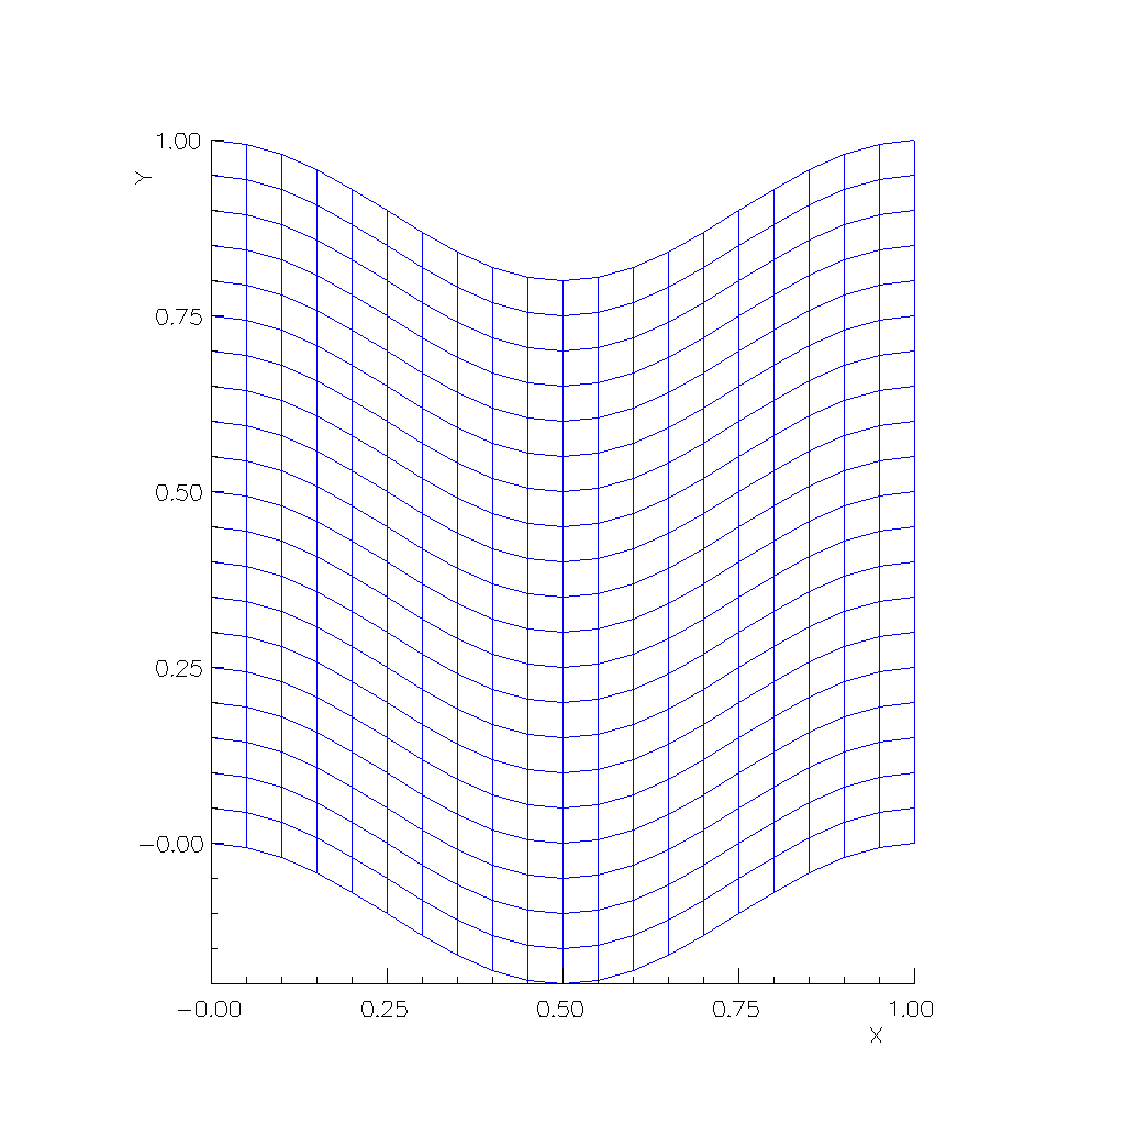
\epsfig{file=sineGrid.ps,width=.45\linewidth}  
\epsfig{file=dsiSine41.t50.ps,width=.45\linewidth}  
\end{center}
\caption{Left: the Sine grid. Right: DSI solution at $t=50$ on a $41\times 41$ grid.}
\end{figure}


\begin{table}[hbt]
\begin{center}
\begin{tabular}{|c|c|c|c|} \hline 
  grid            &   DSI (quad) & NFDTD       &   DSI (tri)   \\   \hline\hline 
  sine 21         & $1.08e+0$   & $1.42e+0$  & $1.5e+0$     \\ 
  sine 41         & $3.13e-1$   & $4.48e-1$  & $1.4e+0$     \\ 
  sine 81         & $8.01e-2$   & $1.16e-1$  & $4.9e-1$     \\ 
  sine 161        & $        $  & $2.90e-2$  & $1.2e-1$     \\ 
   rate           &             &             &                \\ \hline
\end{tabular}
\end{center}
\caption{Two dimensional Maxwell equations. Errors in $E_x$. Convergence results for the sine grid, $t=50.$
       The NFDTD scheme preserves a discrete energy. The DSI (quad) scheme was stable to time $t=1000$.
        The DSI (tri) scheme went unstable at $t\approx 60$ for $sine 41$}
 \label{tab:sine chevron} 
\end{table}


\begin{figure}
\begin{center}
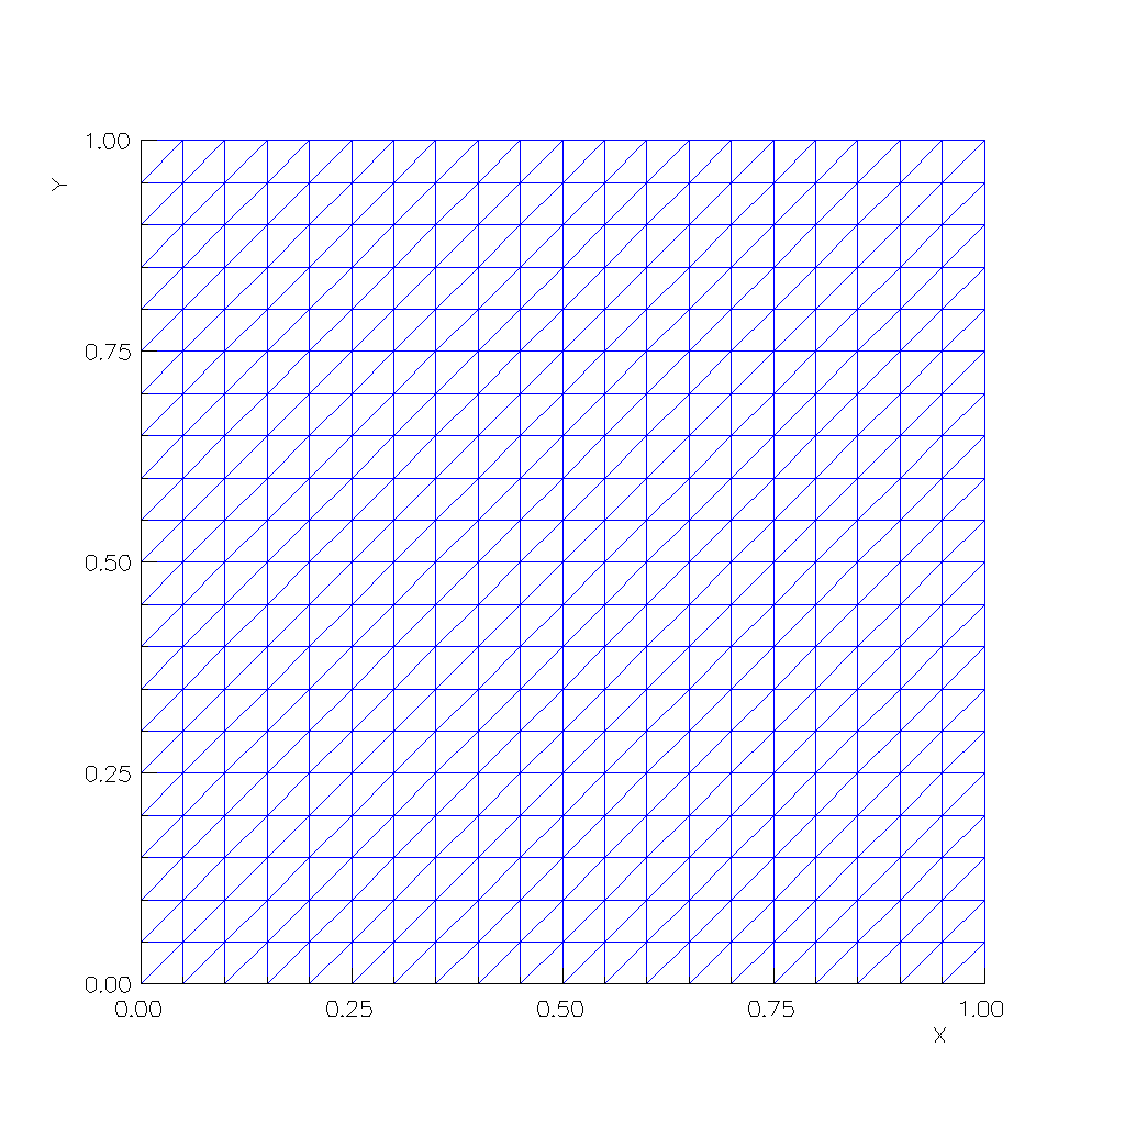
\epsfig{file=sqtriGrid.ps,width=.45\linewidth}  
\epsfig{file=dsiSqTri21.t10.ps,width=.45\linewidth}  
\end{center}
\caption{Left: Unstructured grid of triangles. Right: DSI solution at $t=10.$ on a $21\times 21$ grid.}
\end{figure}

\begin{figure}
\begin{center}
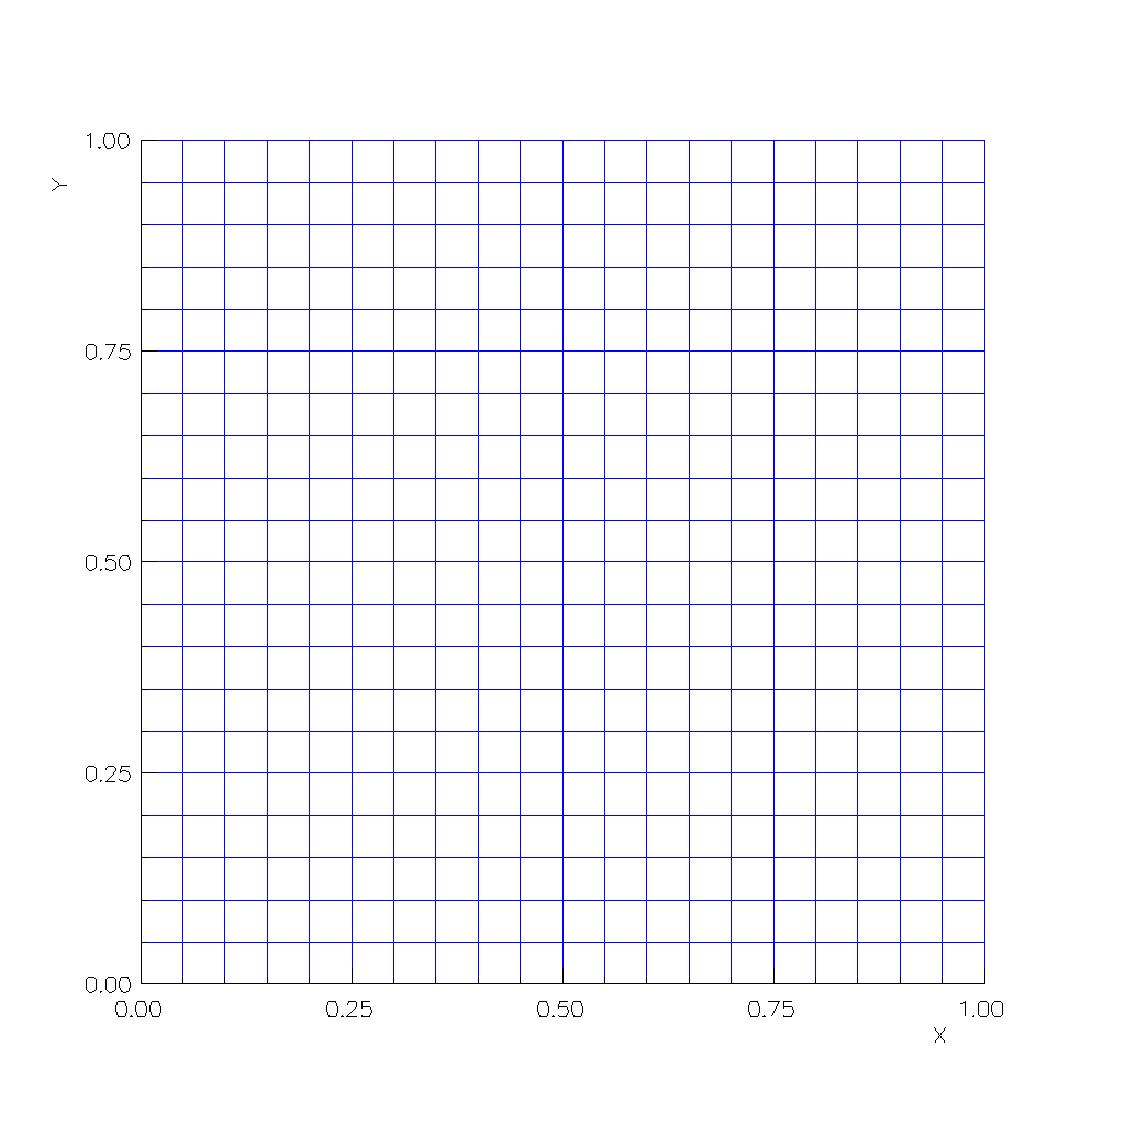
\epsfig{file=sqquadGrid.ps,width=.45\linewidth}  
% \epsfig{file=dsiSqTri41.t50.ps,width=.45\linewidth}  
\end{center}
\caption{Left: Unstructured grid of quadrilaterals. Right: DSI solution at $t=1$ on a $41\times 41$ grid.}
\end{figure}

\begin{figure}
\begin{center}
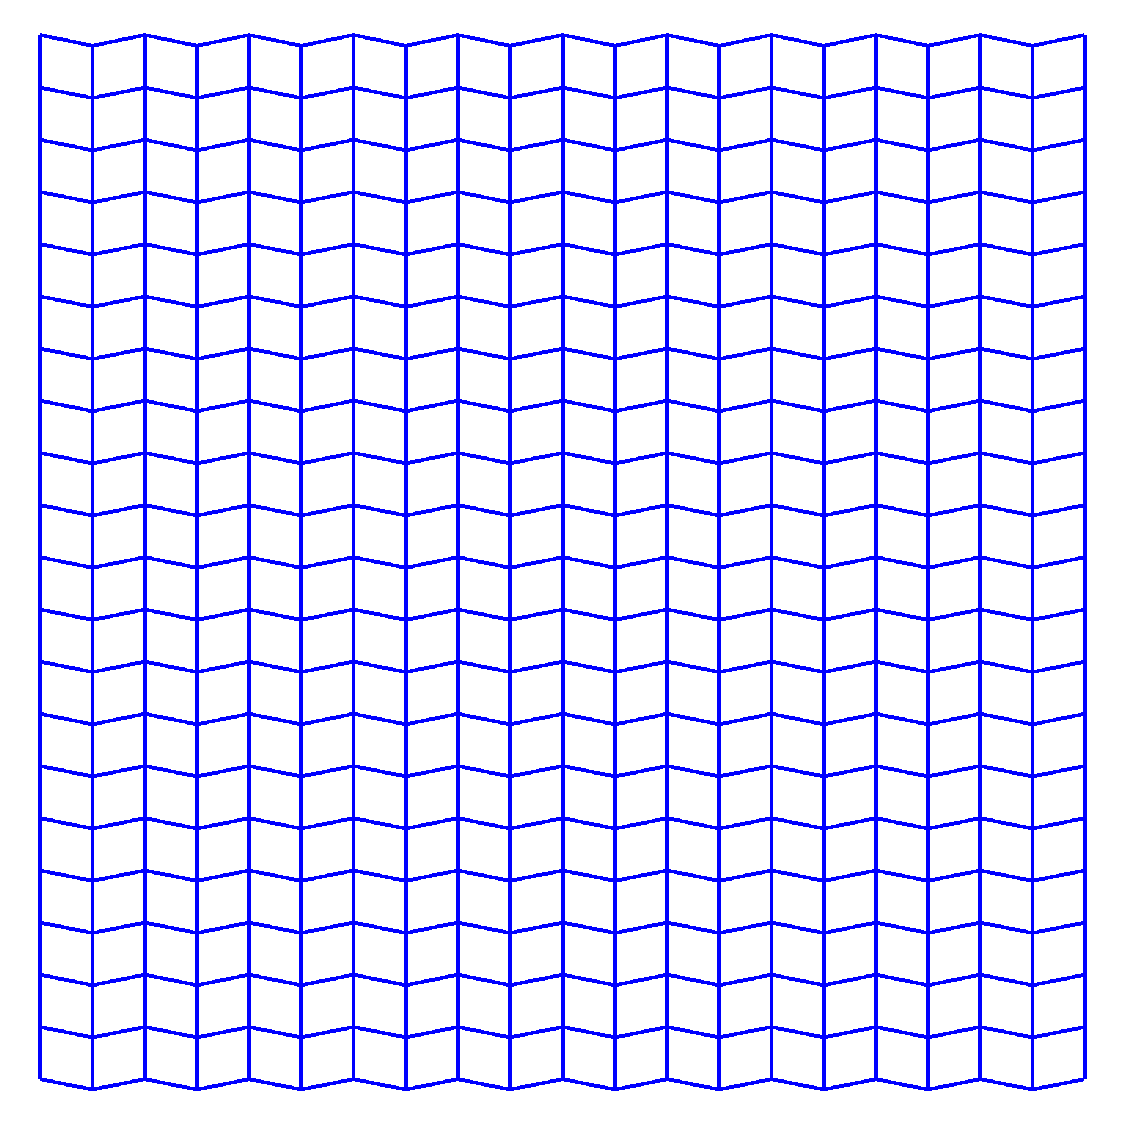
\epsfig{file=chevronGrid.ps,width=.45\linewidth}  
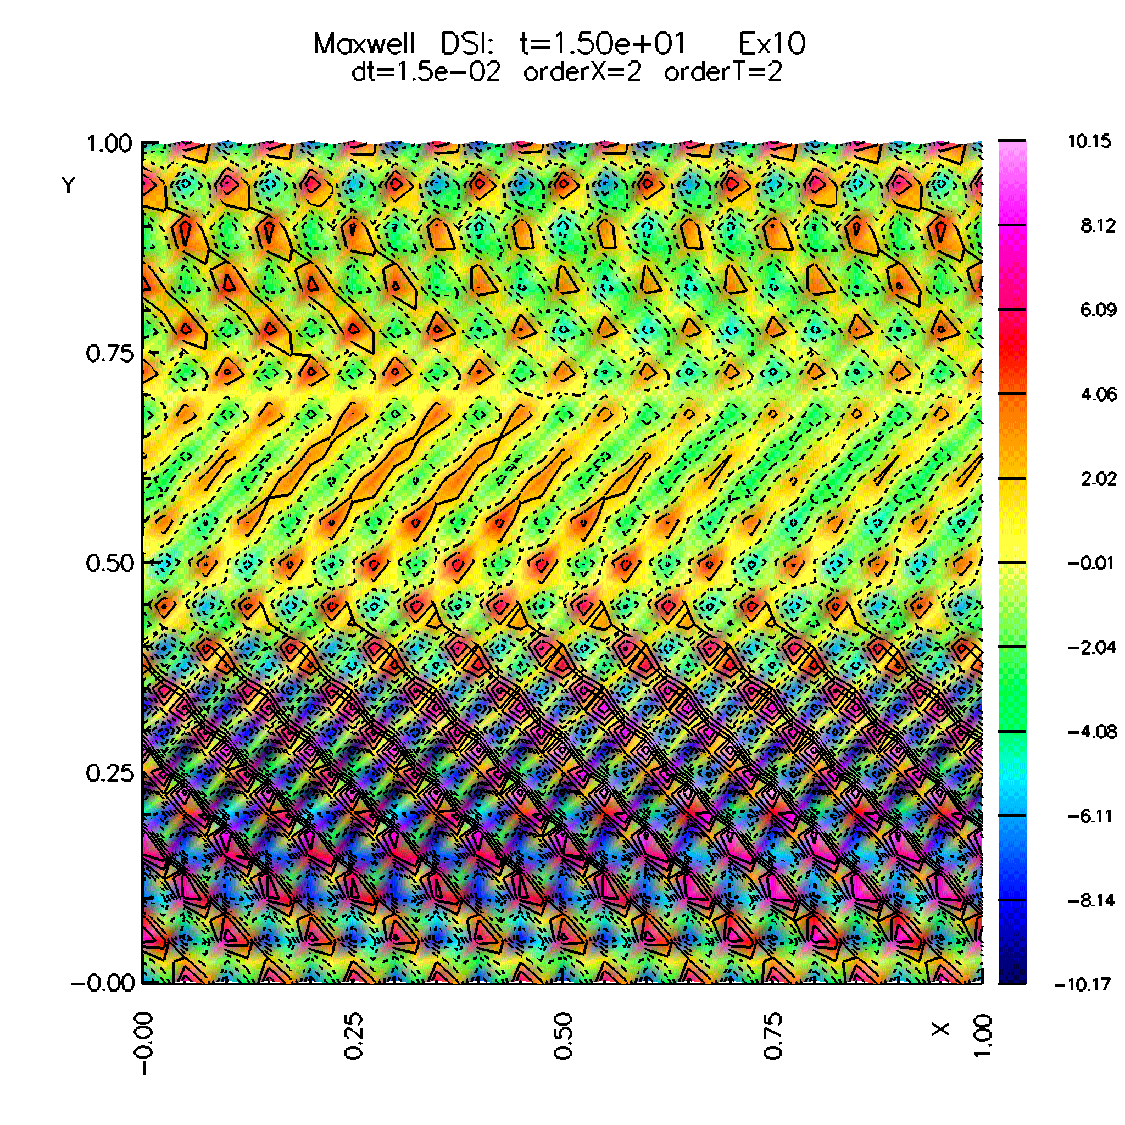
\epsfig{file=dsiChevronUnstable.ps,width=.45\linewidth}  

\end{center}
\caption{Left: the Chevron grid. Right: Unstable solution from the DSI scheme.}
\end{figure}

\begin{figure}
\begin{center}
\epsfig{file=nfdtdChevron41.20.ps,width=.45\linewidth} 
% \end{center}
% \begin{center}
% \vglue-2in
% \begin{minipage}{.4\linewidth}
\vbox{
\begin{tabular}{|c|c|} \hline 
  time   &   ${\cal E}_h$      \\   \hline\hline 
   0     &  $3.9594833e+01$       \\ 
   5     &  $3.9594833e+01$        \\ 
   10    &  $3.9594833e+01$        \\ 
   15    &  $3.9594833e+01$        \\ 
   20    &  $3.9594833e+01$        \\ \hline
\end{tabular}
}
% \end{minipage}
\end{center}
\caption{Top: Solution on the $41\times41$ Chevron grid with the NFDTD scheme. Bottom: 
  The discrete energy is conserved.}
\end{figure}


\clearpage
\section{Convergence results}

\input results.tex

\vfill\eject
\bibliography{\homeHenshaw/papers/henshaw}
\bibliographystyle{siam}

\printindex

\end{document}


% ----------------------------------------------------------------------------------------------------------



